% !TEX ROOT=./main.tex



\section{Numerical Experiments}


% \begin{figure}
% \begin{tabular}{cc}
% 	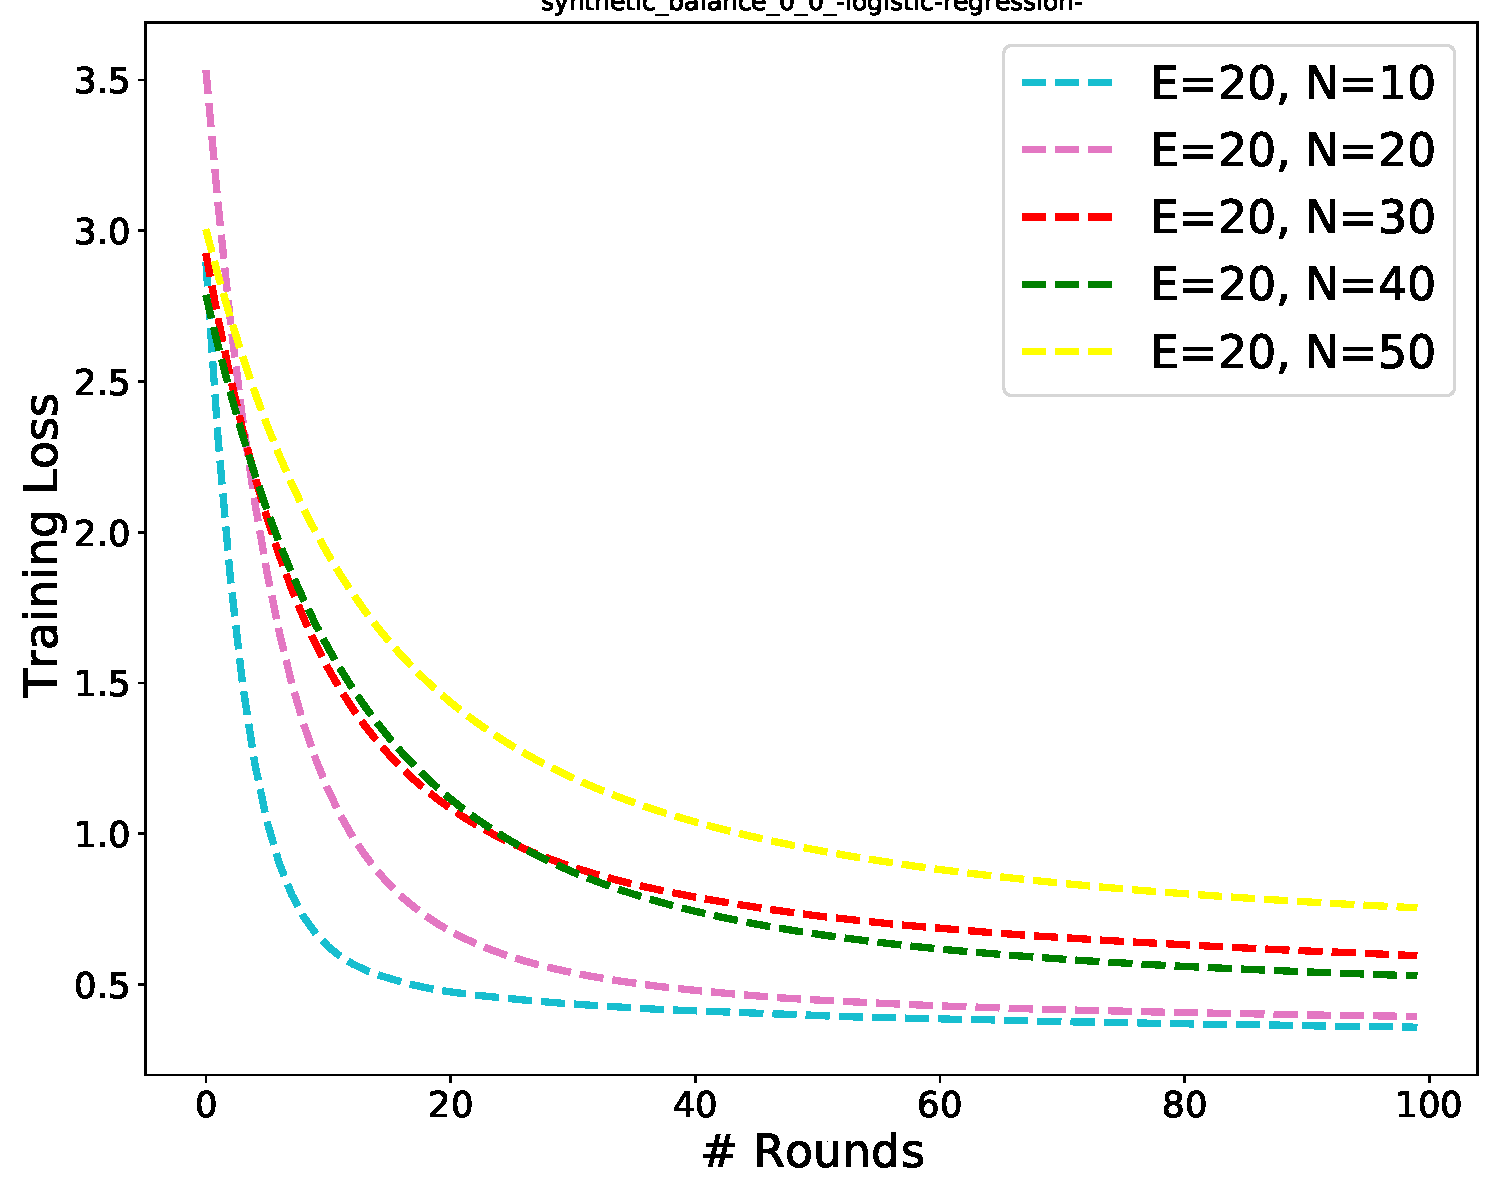
\includegraphics[width=0.5\textwidth]{fig/synthetic_balance_0_0_loss.pdf} & 
% 	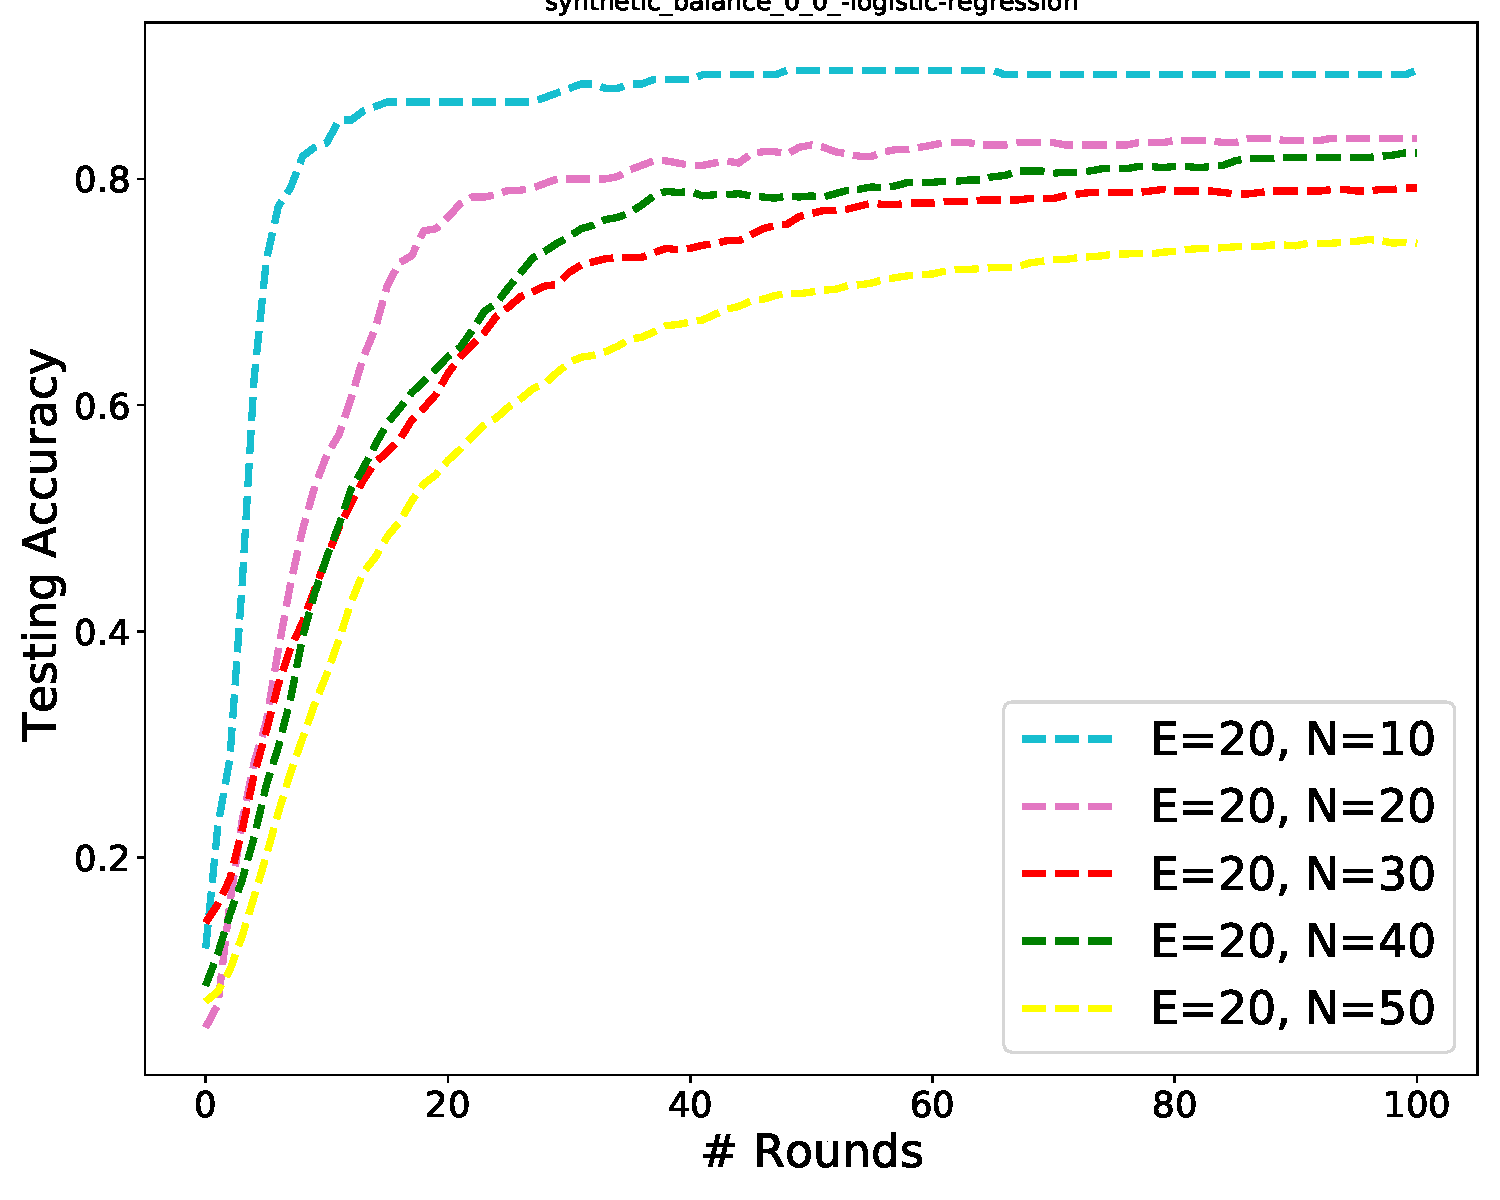
\includegraphics[width=0.5\textwidth]{fig/synthetic_balance_0_0_accuracy.pdf} \\
% 	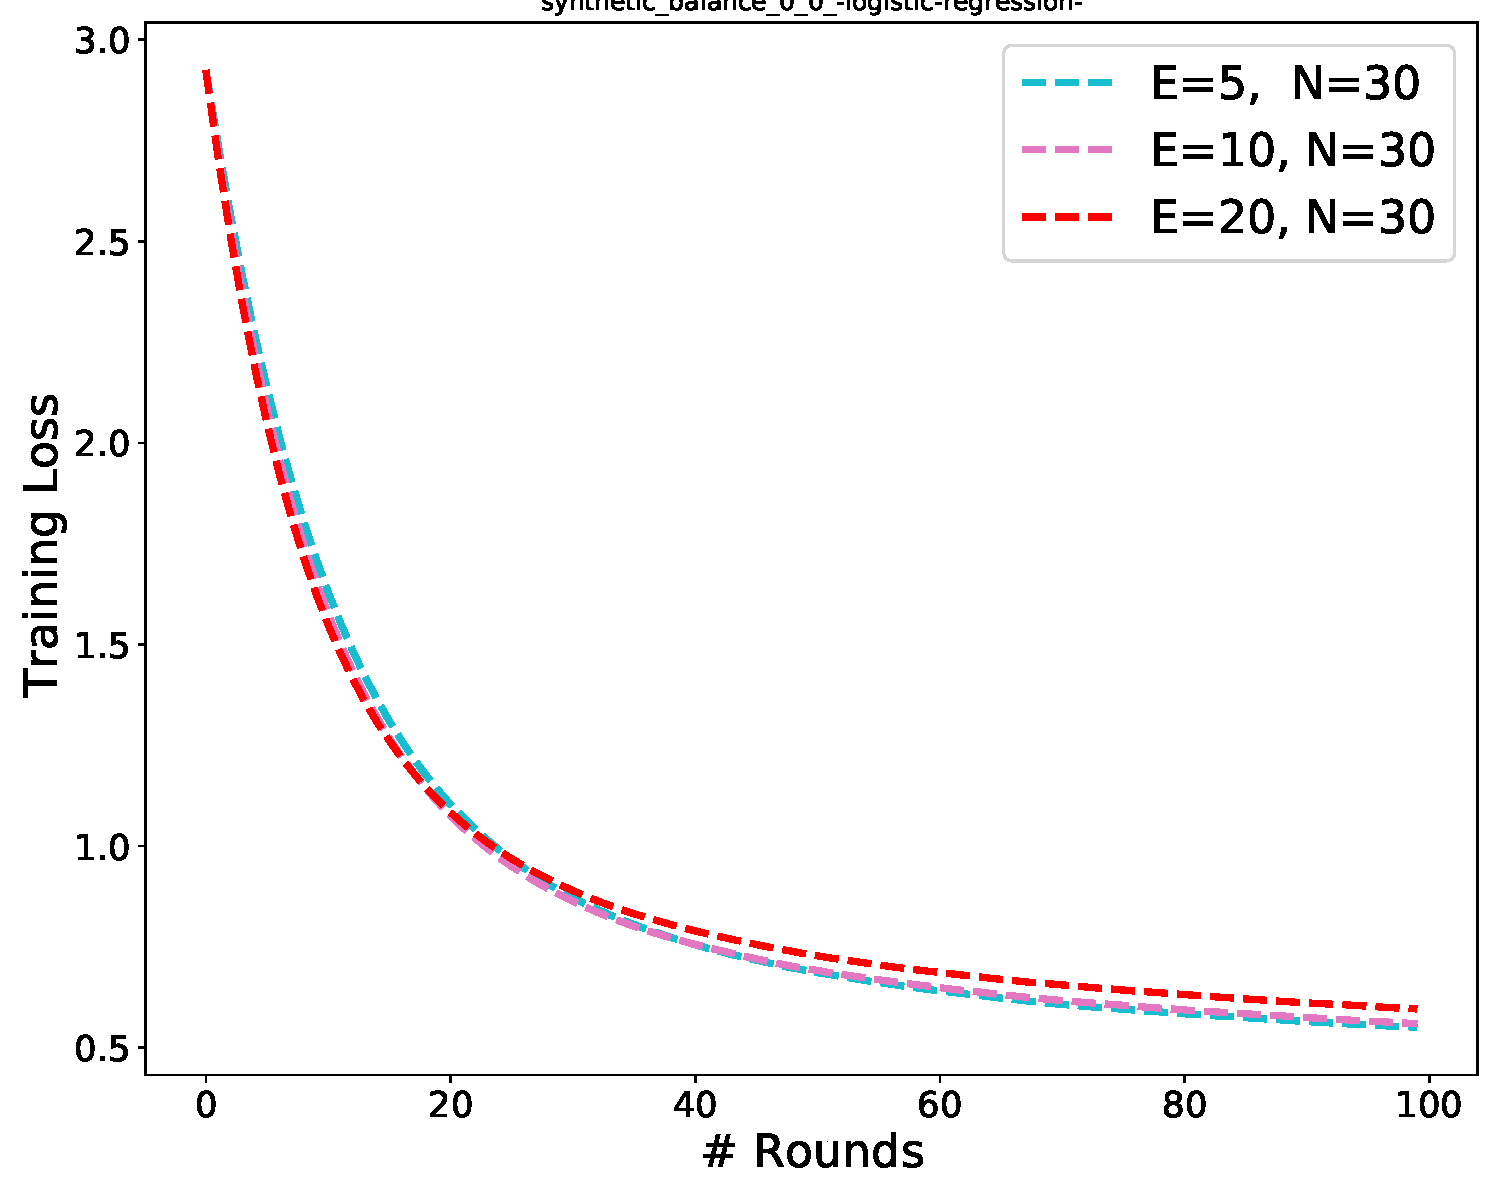
\includegraphics[width=0.5\textwidth]{fig/synthetic_balance_0_0_lossuser30TuneE.pdf} & 
% 	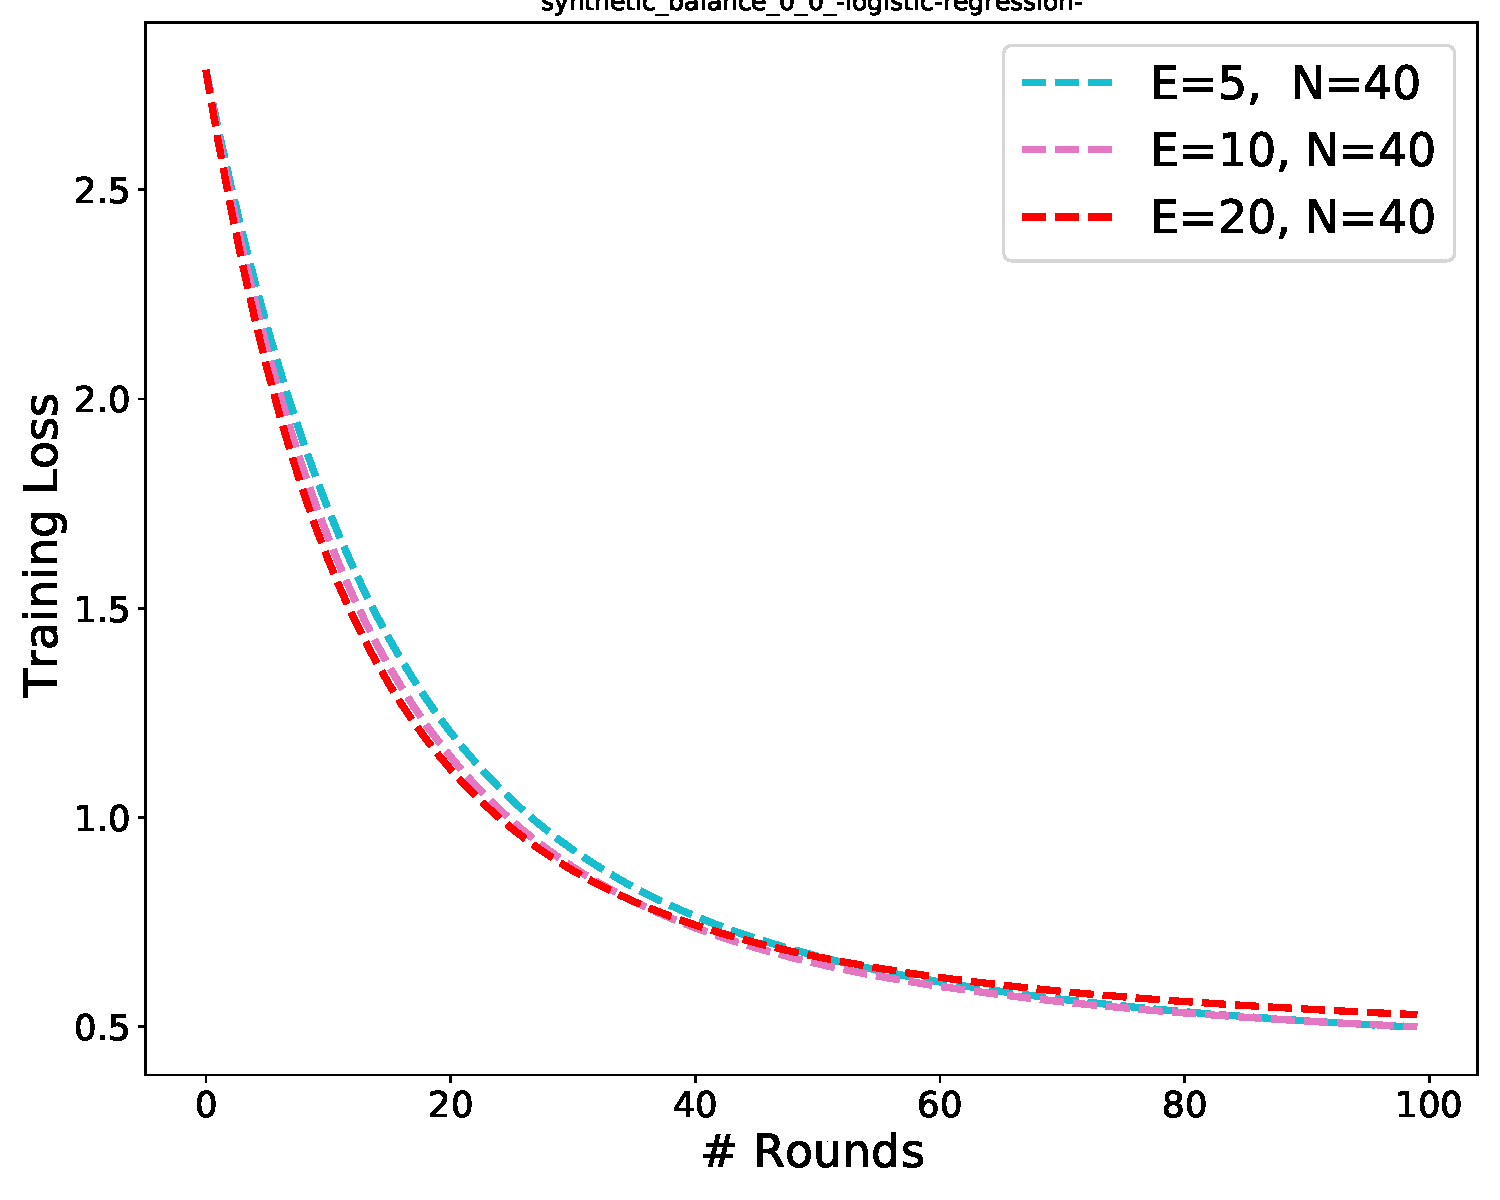
\includegraphics[width=0.5\textwidth]{fig/synthetic_balance_0_0_lossuser40TuneE.pdf} \\
% \end{tabular}
% \caption{Each user has 250 samples, non-iid setting, full device participation. Constant learning rate 0.01.}
% \end{figure}

\subsection{SGD}
We examine the practical speedup on a linear regression problem, 
$ F(\vw) = \sum_{k=1}^N p_kF_k(\vw)$, the objective function on each local device $k$ is given by, $F_k(\vw) = \frac{1}{N_k} \sum_{i=1}^{N_k} (\vw^T\vx_i^k + b  - y_i^k)^2$, where we generated i.i.d. data $\vx_i^k$ for all devices. At each communication round, all devices participated
in synchronization. 

\begin{figure}
\centering
\begin{tabular}{cc}
	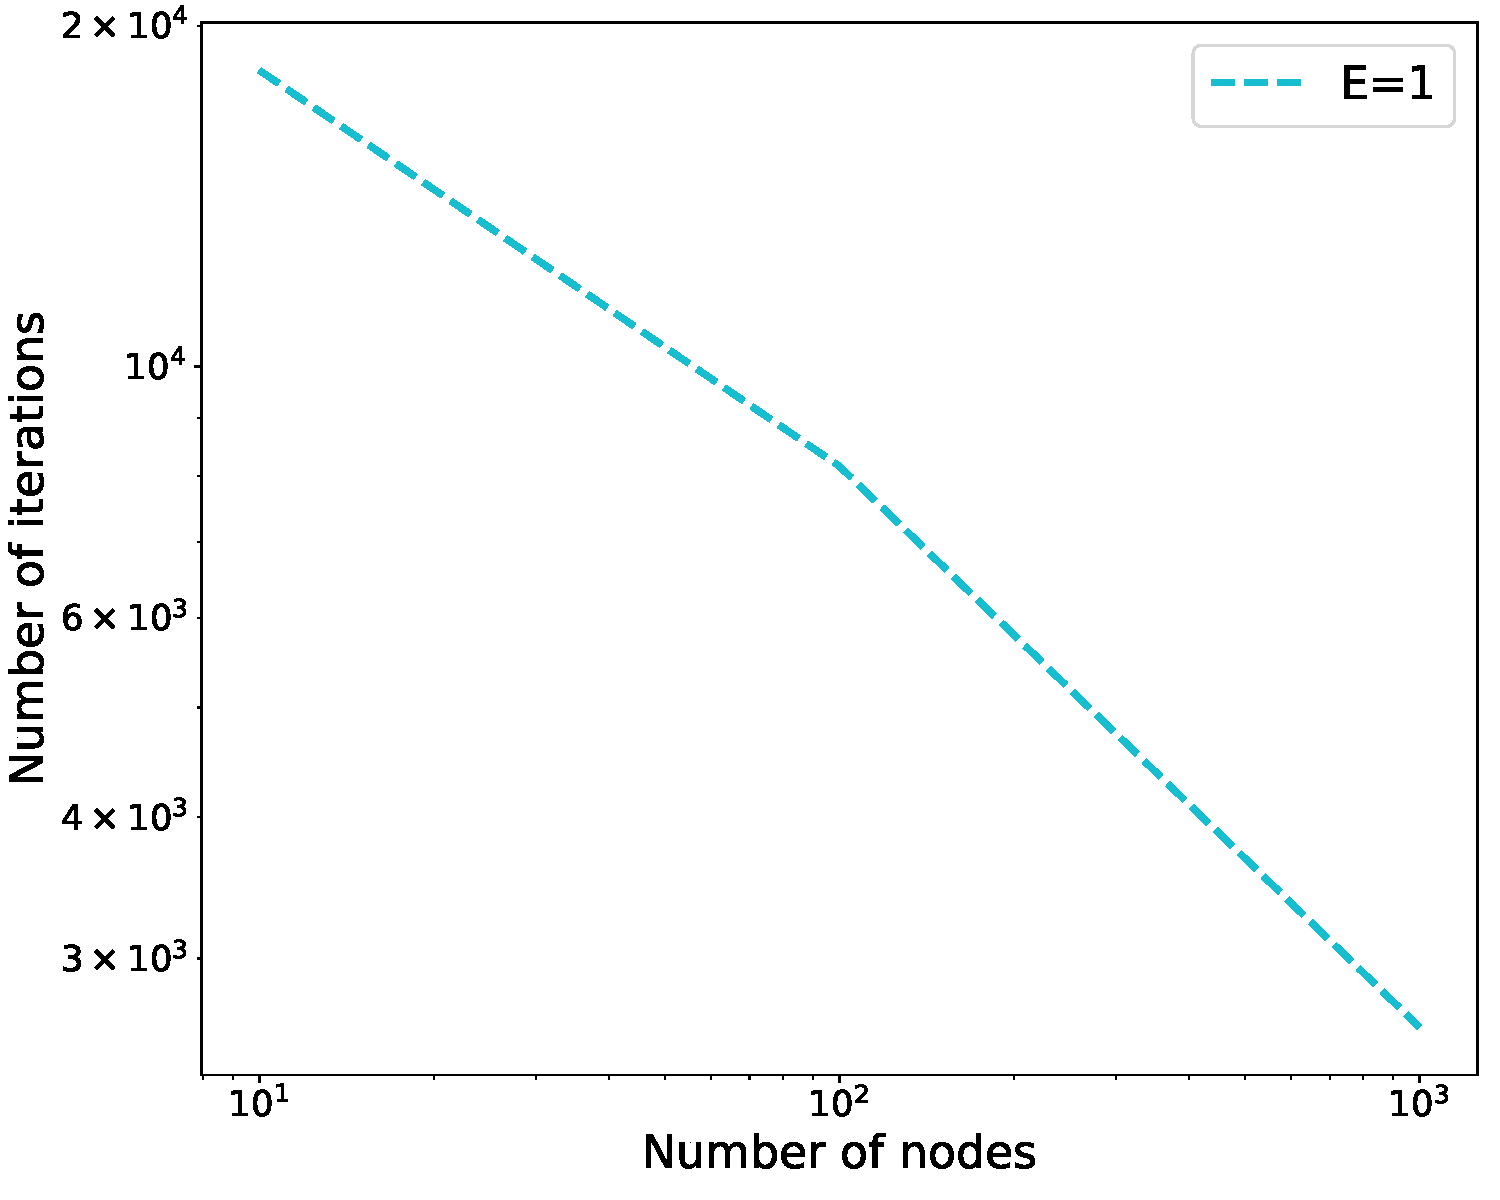
\includegraphics[width=0.5\textwidth]{fig/synthetic_linear_regression_1k_6k-epsilon01-logTrue.pdf} & 
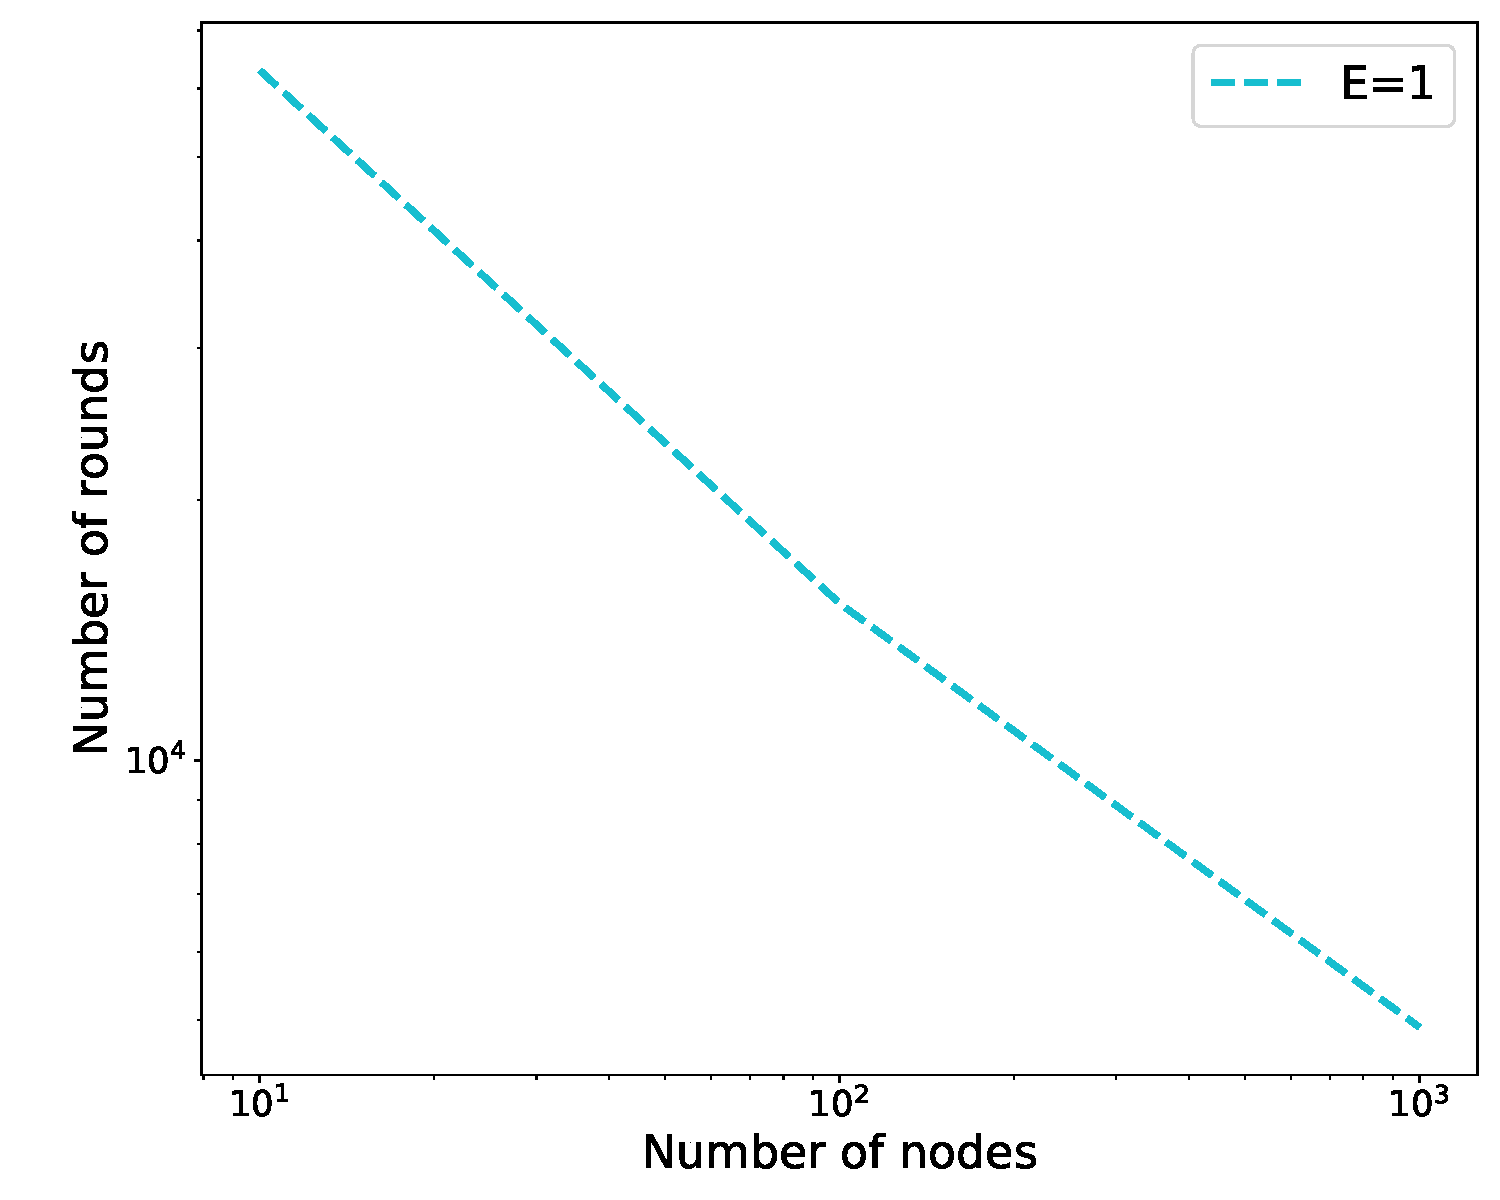
\includegraphics[width=0.5\textwidth]{fig/synthetic_linear_regression_1k_6k-epsilon001-logTrue-epoch-1.pdf} \\
(a) $\epsilon=0.01$  & (b) $\epsilon=0.001$
\end{tabular}
	\caption{The linear speed up w.r.t the number of nodes. The synthetic dataset has $6000$ samples, evenly distributed on $10, 50, 100, 500, 1000$ devices. The figure shows the number of iterations needed to converge to $\epsilon$. The learning rate is decayed as the $\eta_t = \frac{1}{c + t \times a}$, where we extensively search the best learning rate $c \in \{1, 10\}$ and $a \in \{1\mathrm{e}{-2}, 1\mathrm{e}{-3}, 1\mathrm{e}{-4}, 1\mathrm{e}{-5}, 1\mathrm{e}{-6}\}$ for each configuration. Batch size is 6 in this case.}
\end{figure}

\begin{figure}
\centering
\begin{tabular}{cc}
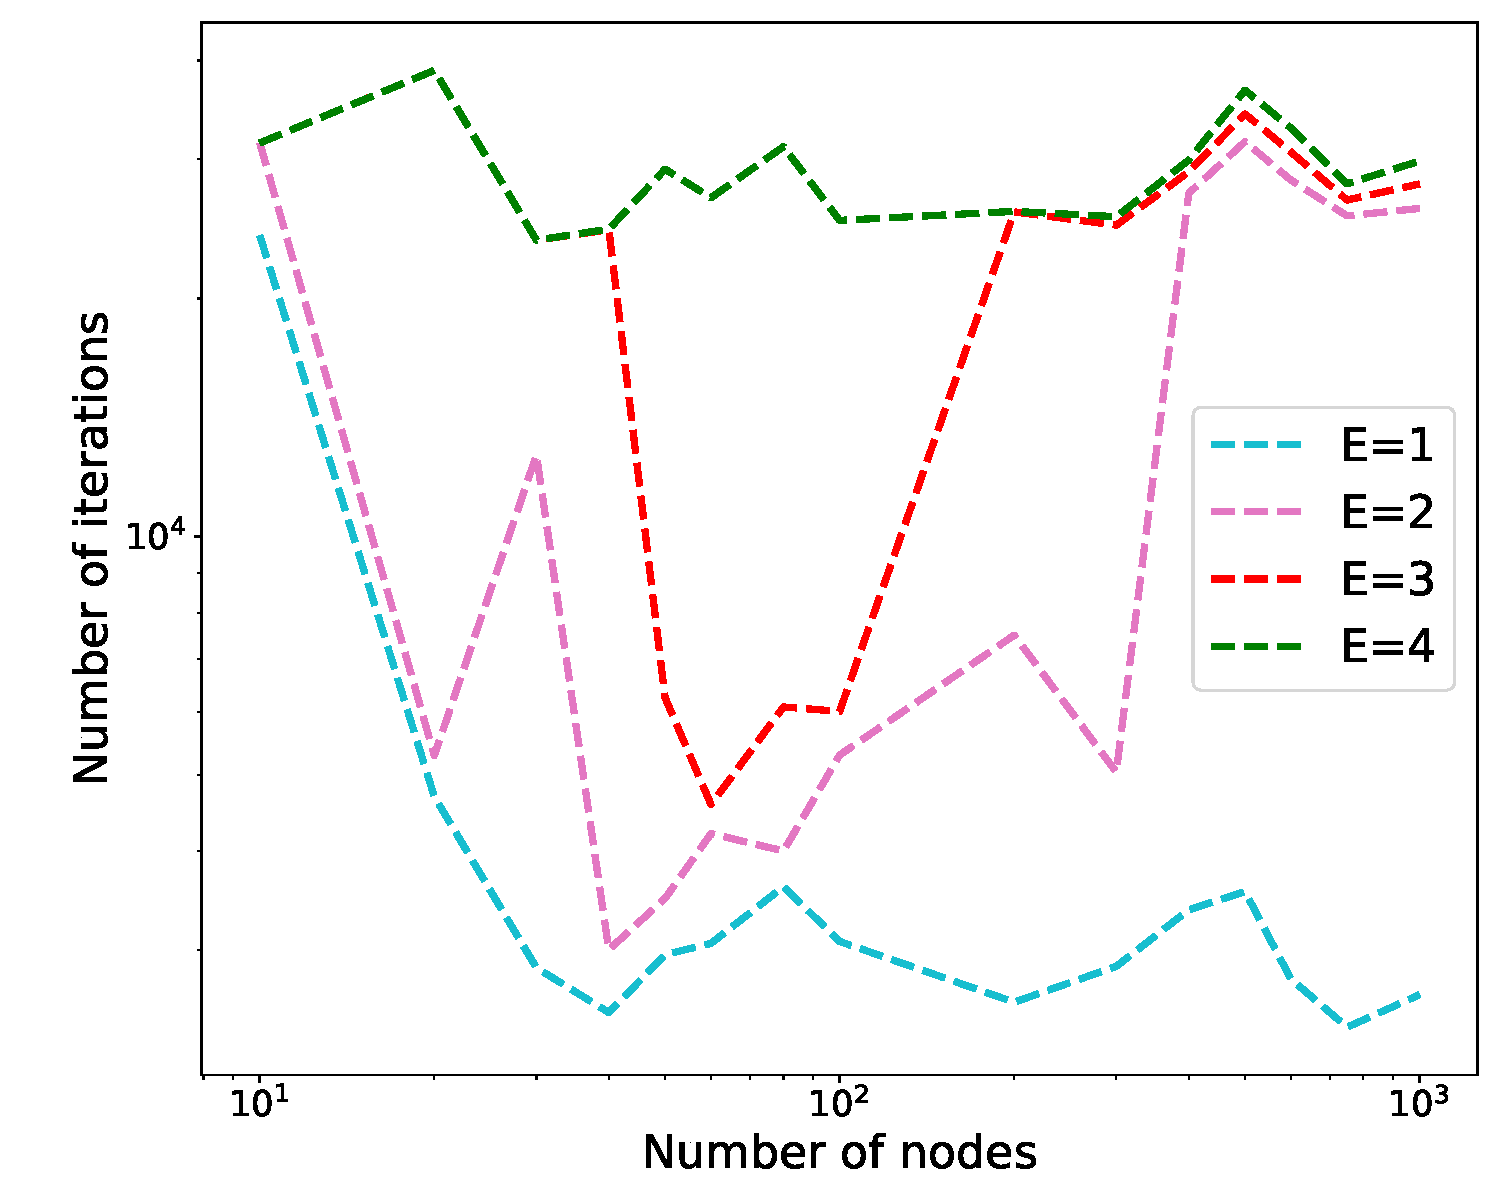
\includegraphics[width=0.5\textwidth]{fig/synthetic_linear_regression_1k_6k-epsilon001-logTrue-epoch-1-2-3-4-b4-adapt0.pdf} & 
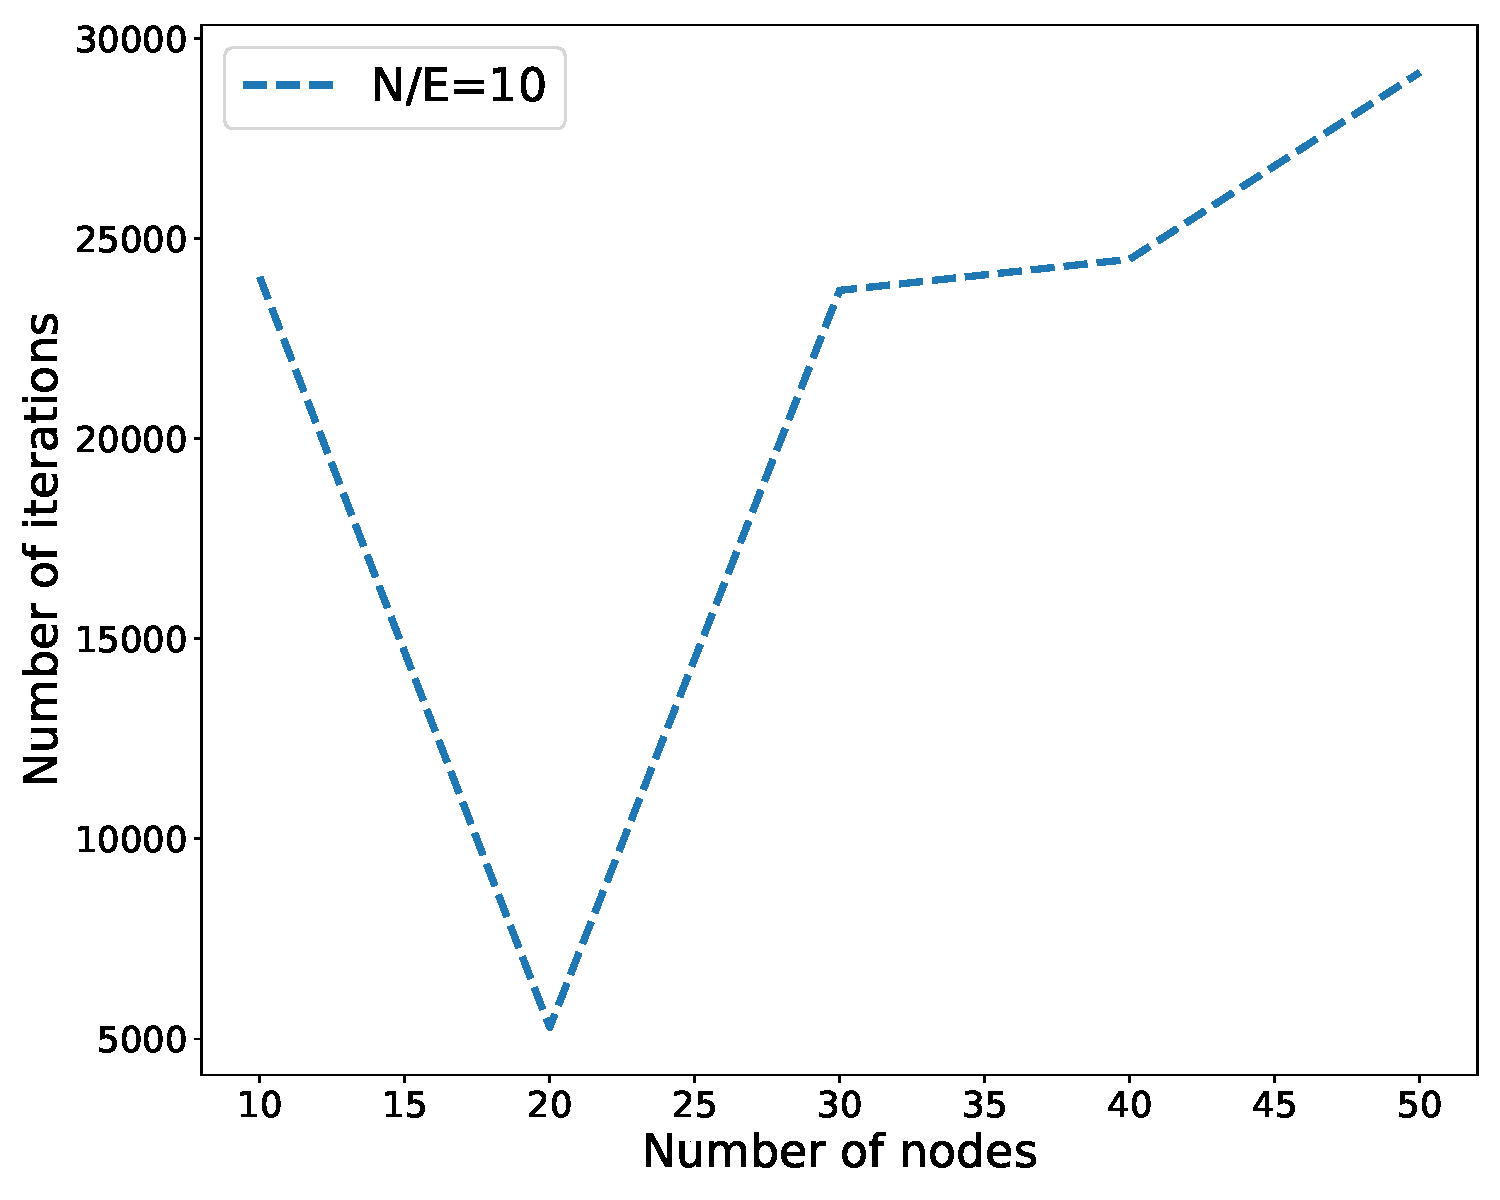
\includegraphics[width=0.5\textwidth]{fig/iteration_EandN-synthetic_linear_regression_1k_6k-epsilon01.pdf} 
 \\
(a) $\epsilon=0.01$  & (b) $N/E = 10$ 
\end{tabular}
	\caption{linear regression. The linear speed up w.r.t the number of nodes. The synthetic dataset has $6000$ samples, evenly distributed on $10, 20, 30, 40, 50, 60, 80, 100, 200, 300, 400, 500, 600, 750, 1000$ devices. The figure shows the number of iterations needed to converge to $\epsilon$. The learning rate is decayed as the $\eta_t = \frac{1}{c + t \times a}$, where we extensively search the best learning rate $c \in \{1, 10\}$ and $a \in \{1\mathrm{e}{-2}, 1\mathrm{e}{-3}, 1\mathrm{e}{-4}, 1\mathrm{e}{-5}, 1\mathrm{e}{-6}\}$ for each configuration. Batch size is 4 in this case.}
\end{figure}


\begin{figure}
\centering
% \begin{tabular}{cc}
% 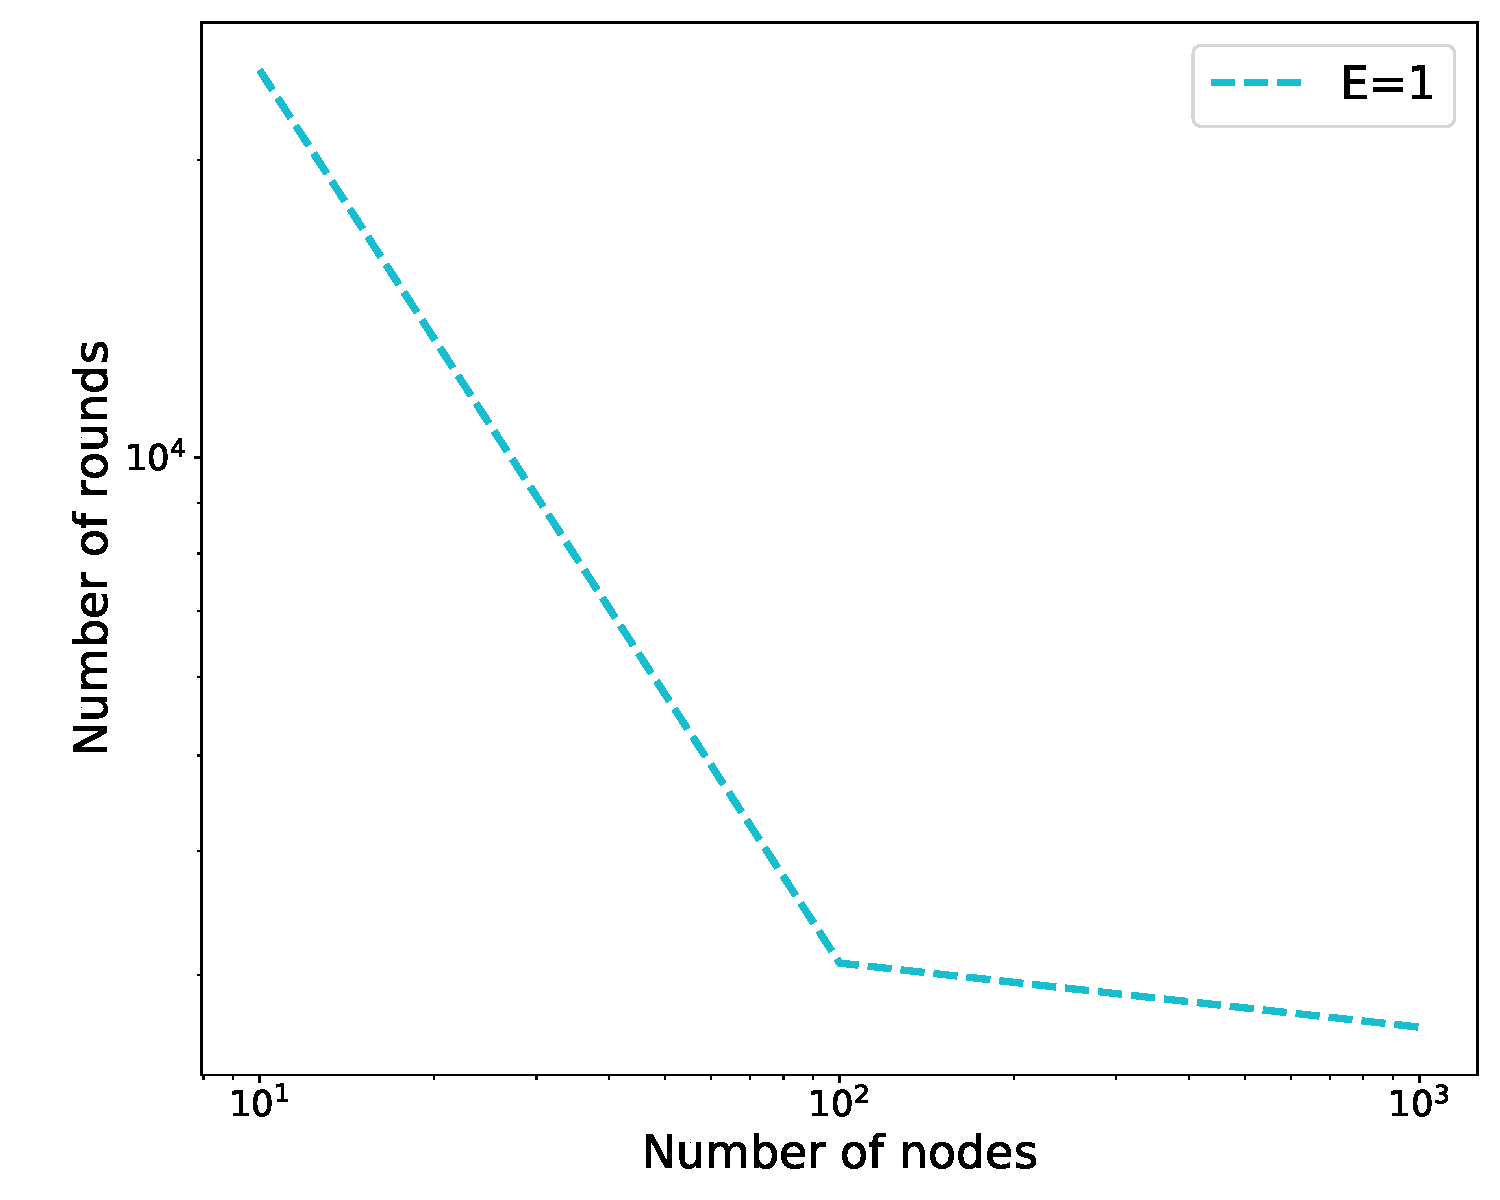
\includegraphics[width=0.5\textwidth]{fig/synthetic_linear_regression_noise1e-02-epsilon1e-02-logTrue-epoch-1-b4} \\ 
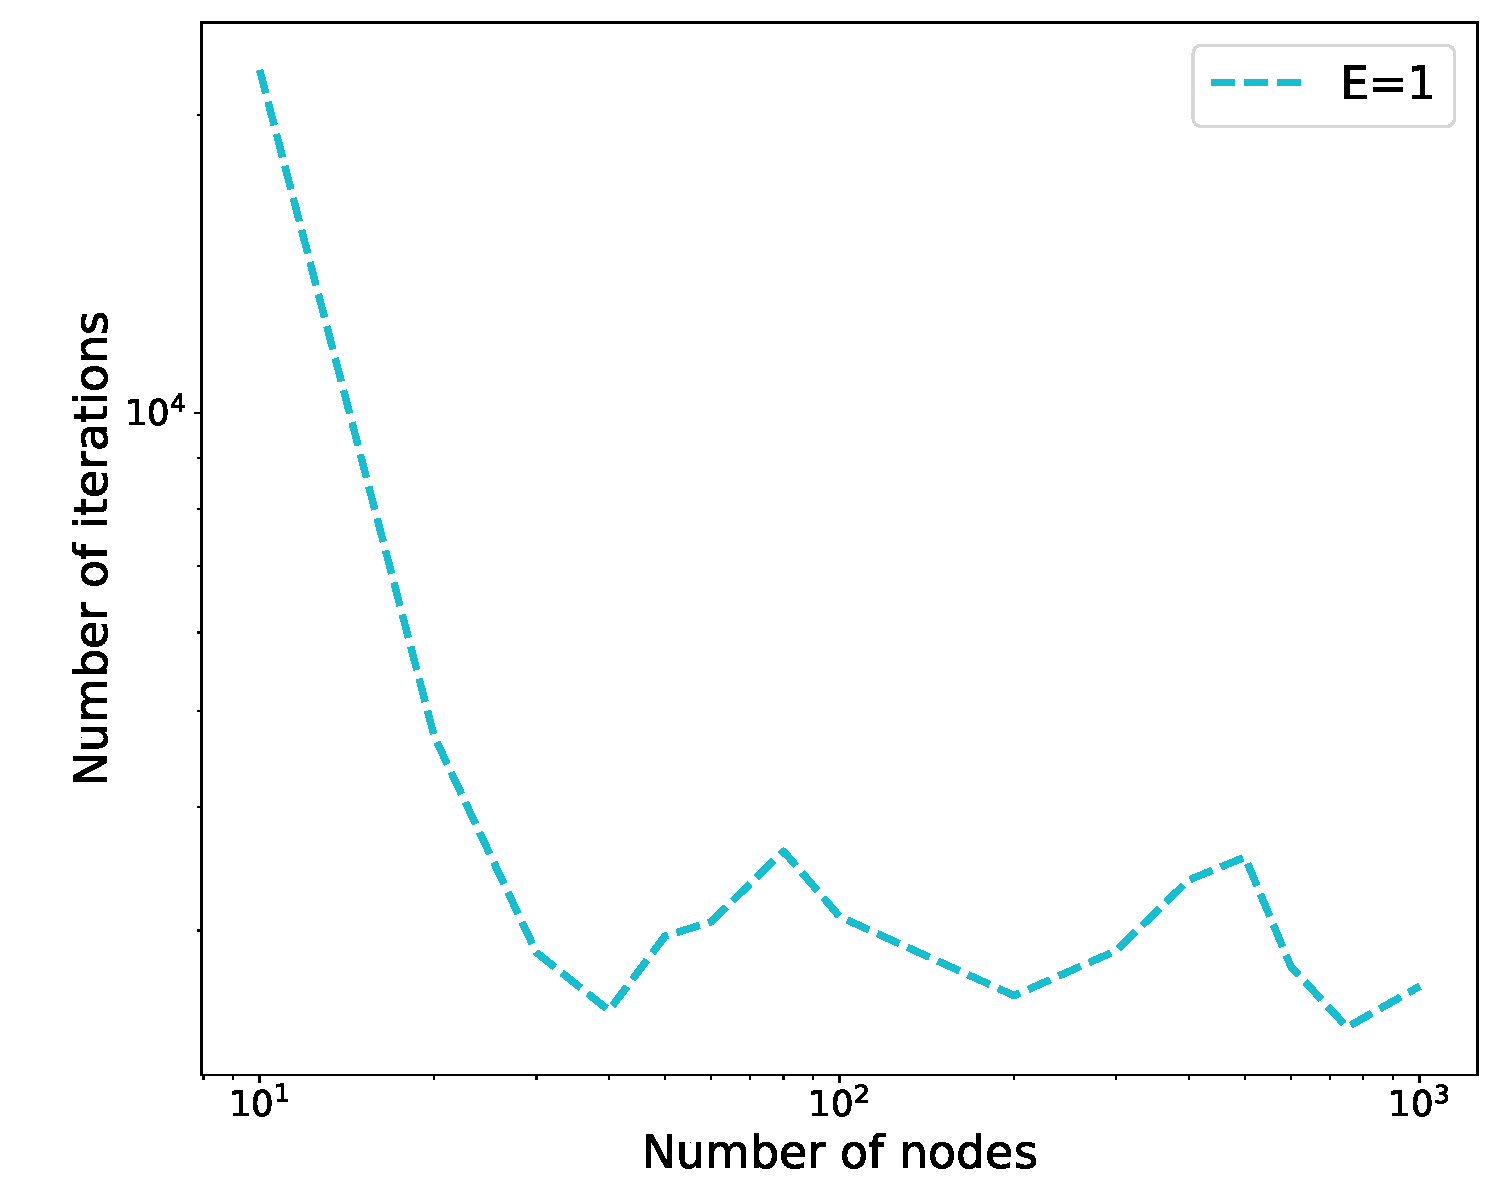
\includegraphics[width=0.5\textwidth]{fig/synthetic_linear_regression_noise1e-02-epsilon01008-logTrue-epoch-1-b4-adapt0.pdf} \\ 
% \end{tabular}
(a) $\epsilon=0.01$ \\
	\caption{The linear speed up w.r.t the number of nodes. The synthetic dataset has $6000$ samples, evenly distributed on $10, 20, 30, 40, 50, 60, 80, 100, 200, 300, 400, 500, 600, 750, 1000$ devices. The figure shows the number of iterations needed to converge to $\epsilon$. The learning rate is decayed as the $\eta_t = \frac{1}{c + t \times a}$, where we extensively search the best learning rate $c \in \{1, 10\}$ and $a \in \{1\mathrm{e}{-2}, 1\mathrm{e}{-3}, 1\mathrm{e}{-4}, 1\mathrm{e}{-5}, 1\mathrm{e}{-6}\}$ for each configuration. Batch size is 4 in this case. 
	We add Gaussian noise with zero mean and 0.01 standard deviation.}
\end{figure}


What is the relationship between $N/E$ and iteration $T$ in strongly convex function? $linear regression$, no noise. 
\begin{itemize}
	\item $N/E = 10$
	\item $N=10, E=1$, $N=20, E=2$, $N=30, E=3$, $N=40, E=4$, $N=50, E=5$, $N=100, E=10$.
\end{itemize} 


Does convex smooth function have linear speedup?

\begin{figure}
\centering
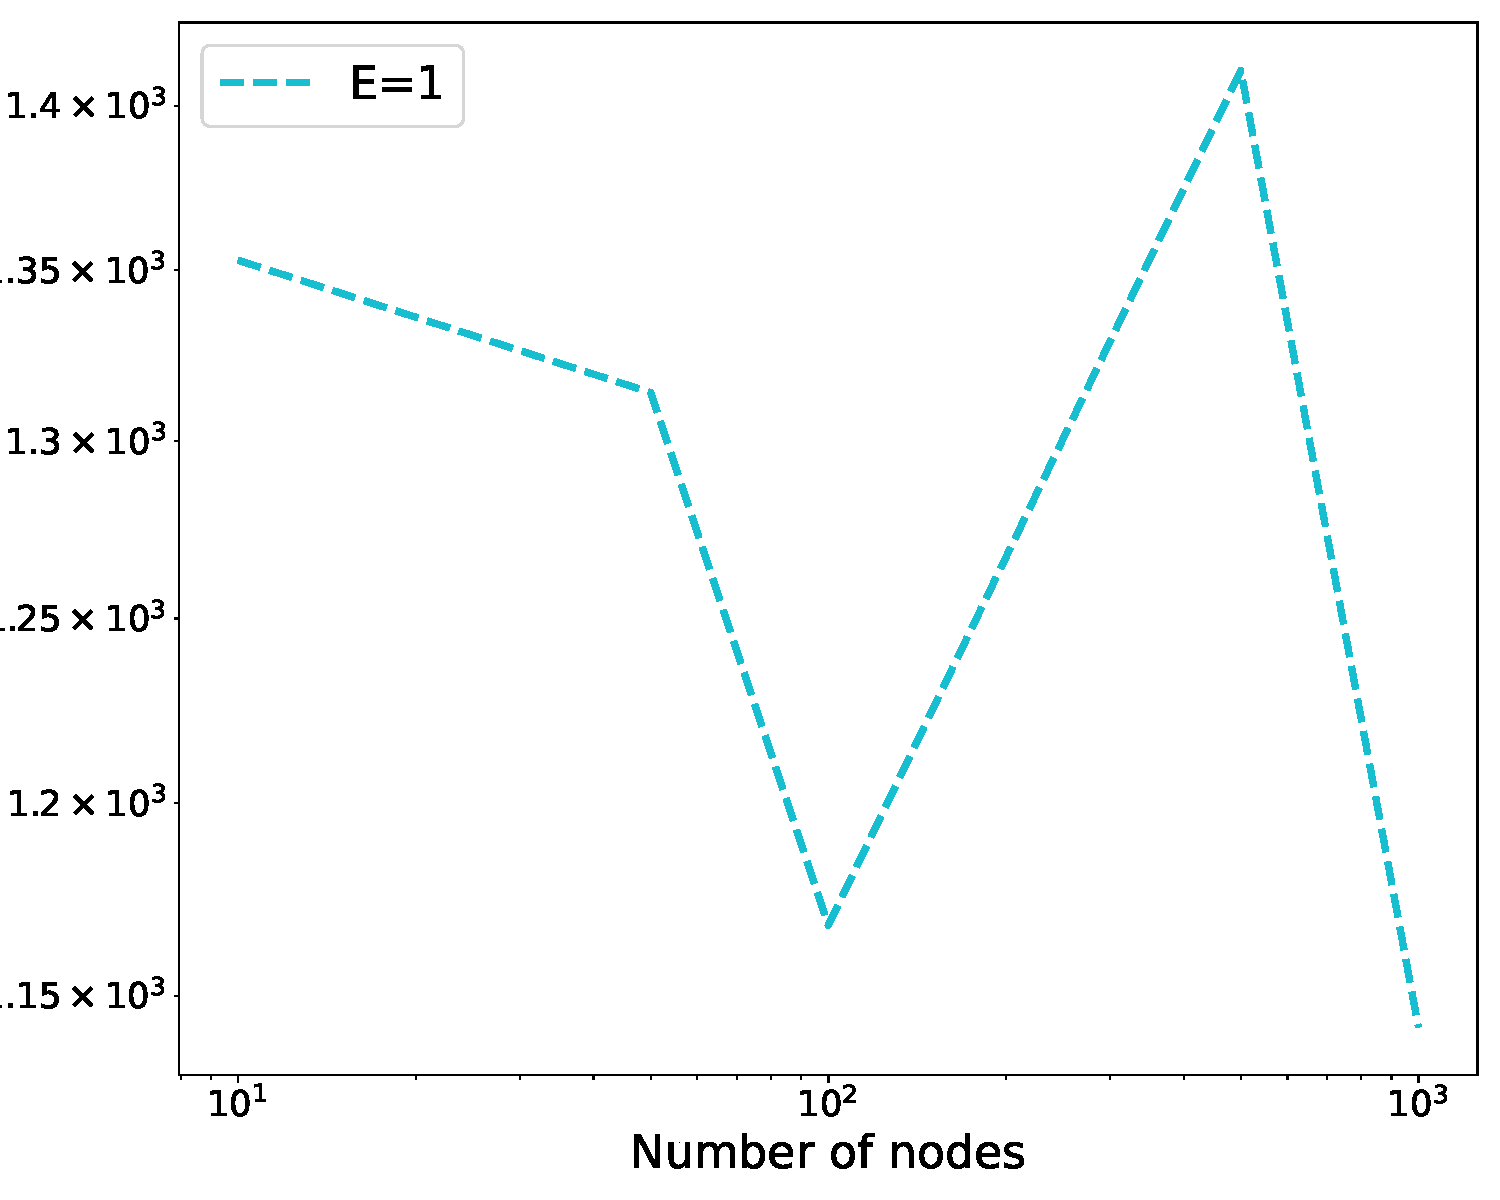
\includegraphics[width=0.5\textwidth]{fig/synthetic_logistic_regression_small-epsilon09-logTrue-epoch-1-b4-regularization0.pdf} \\ 
(a) $\epsilon=0.9$ \\
\caption{Convex smooth objectives (logistic regression with zero l2-regularization) The number of iterations w.r.t the number of nodes. The synthetic dataset has $6000$ samples, evenly distributed on $10, 50, 100, 500, 1000$ devices. The figure shows the number of iterations needed to converge to $\epsilon-$accuracy. The learning rate is decayed as the $\eta_t = \frac{1}{c + t \times a}$, where we extensively search the best learning rate $c \in \{1, 10\}$ and $a \in \{1\mathrm{e}{-2}, 1\mathrm{e}{-3}, 1\mathrm{e}{-4}, 1\mathrm{e}{-5}, 1\mathrm{e}{-6}\}$ for each configuration. Batch size is 4 in this case.}
\end{figure}




\begin{figure}
\centering
\begin{tabular}{cc}
	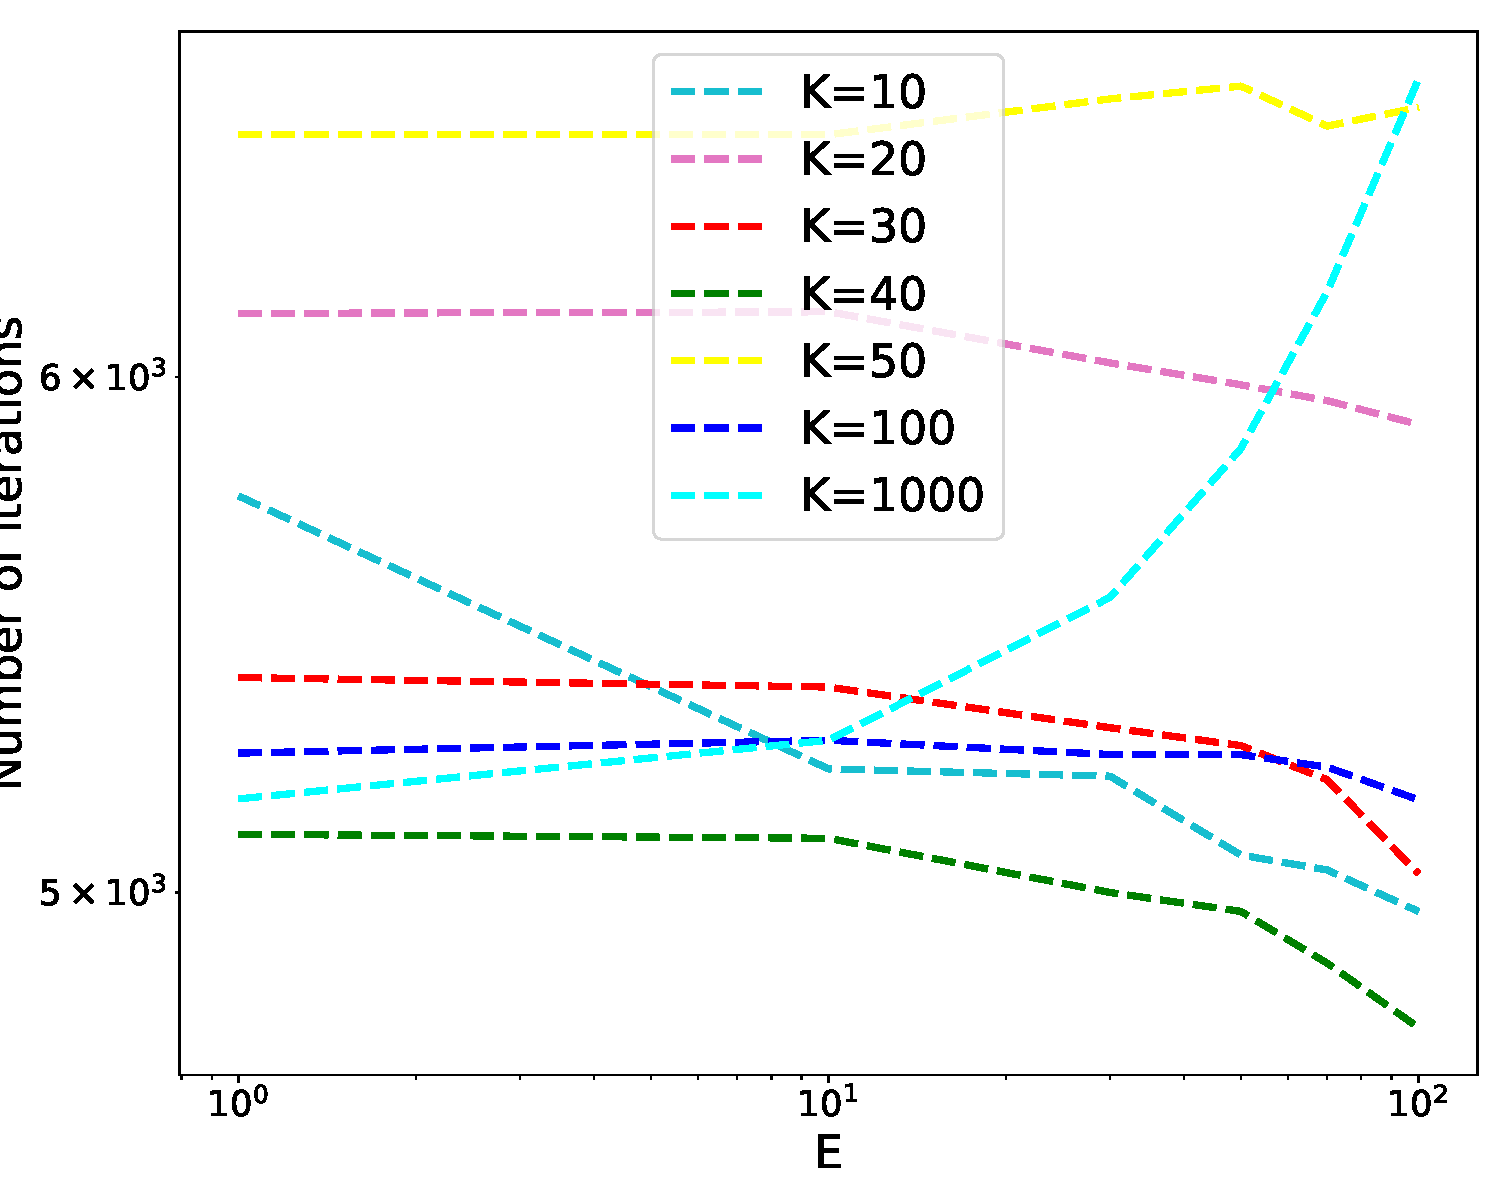
\includegraphics[width=0.5\textwidth]{fig/speedupEpochsT-synthetic_logistic_regression_iclr300-epsilon07-b4-adapt0.pdf} & 
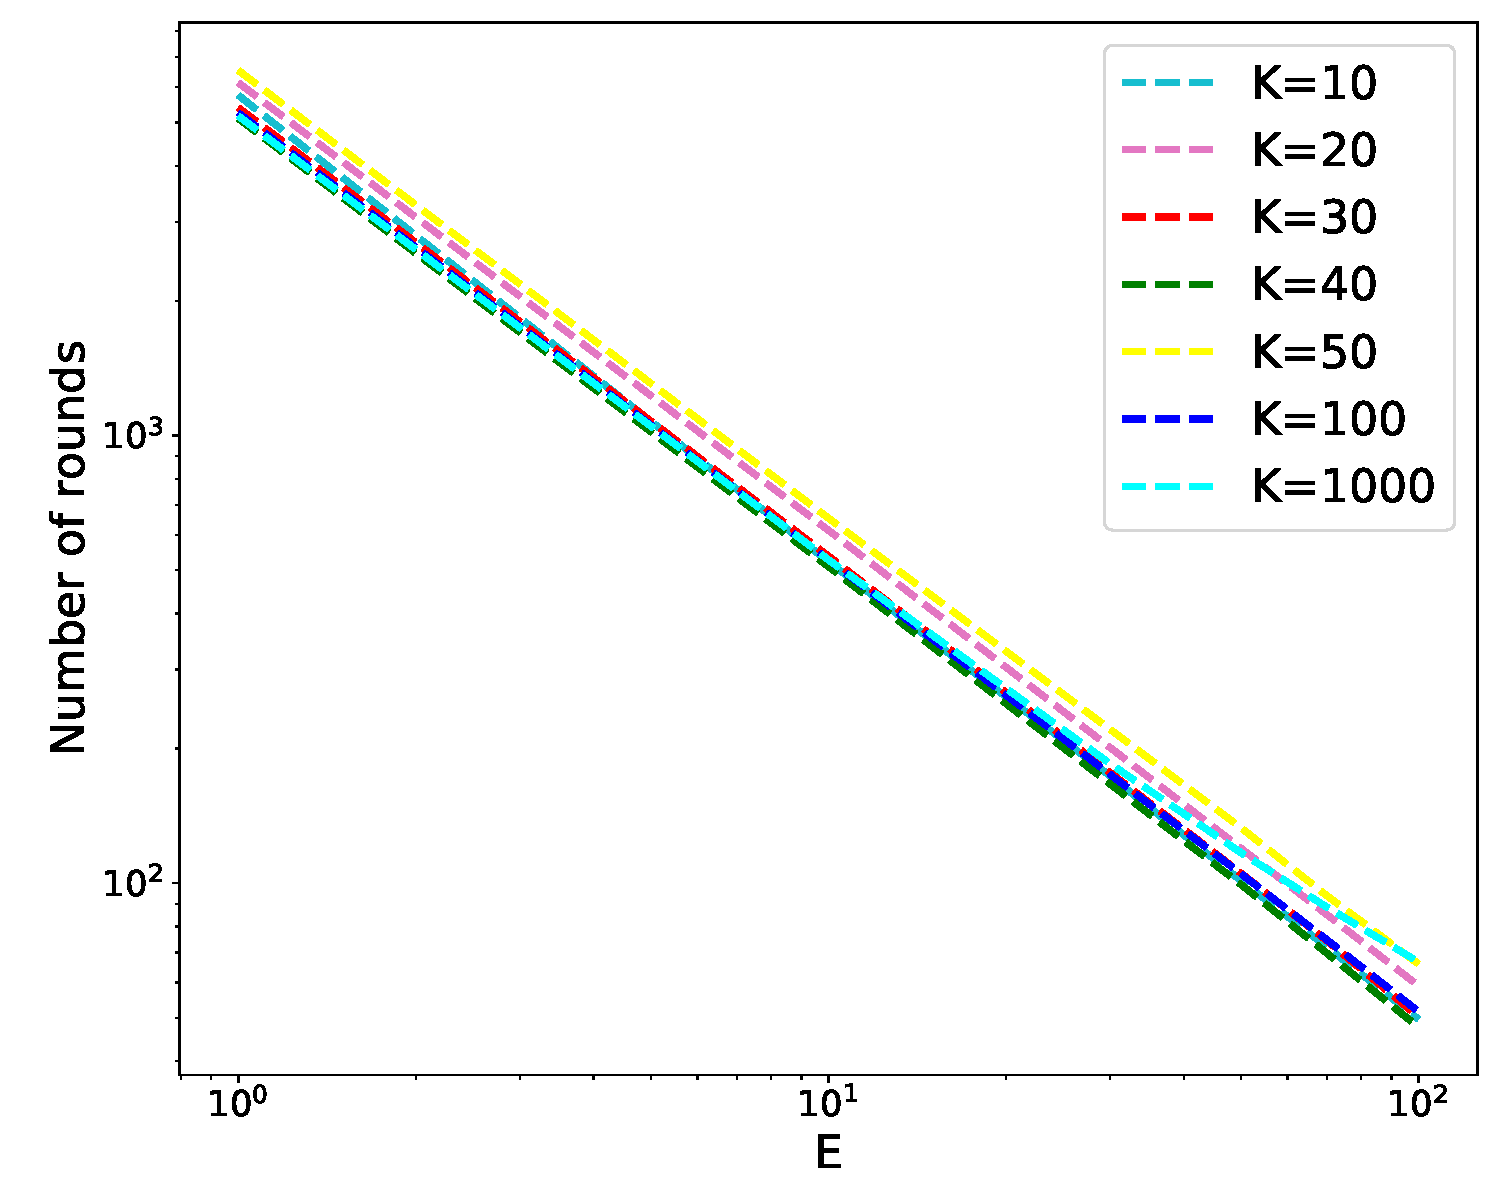
\includegraphics[width=0.5\textwidth]{fig/speedupEpochsRounds-synthetic_logistic_regression_iclr300-epsilon07-b4-adapt0.pdf} \\
	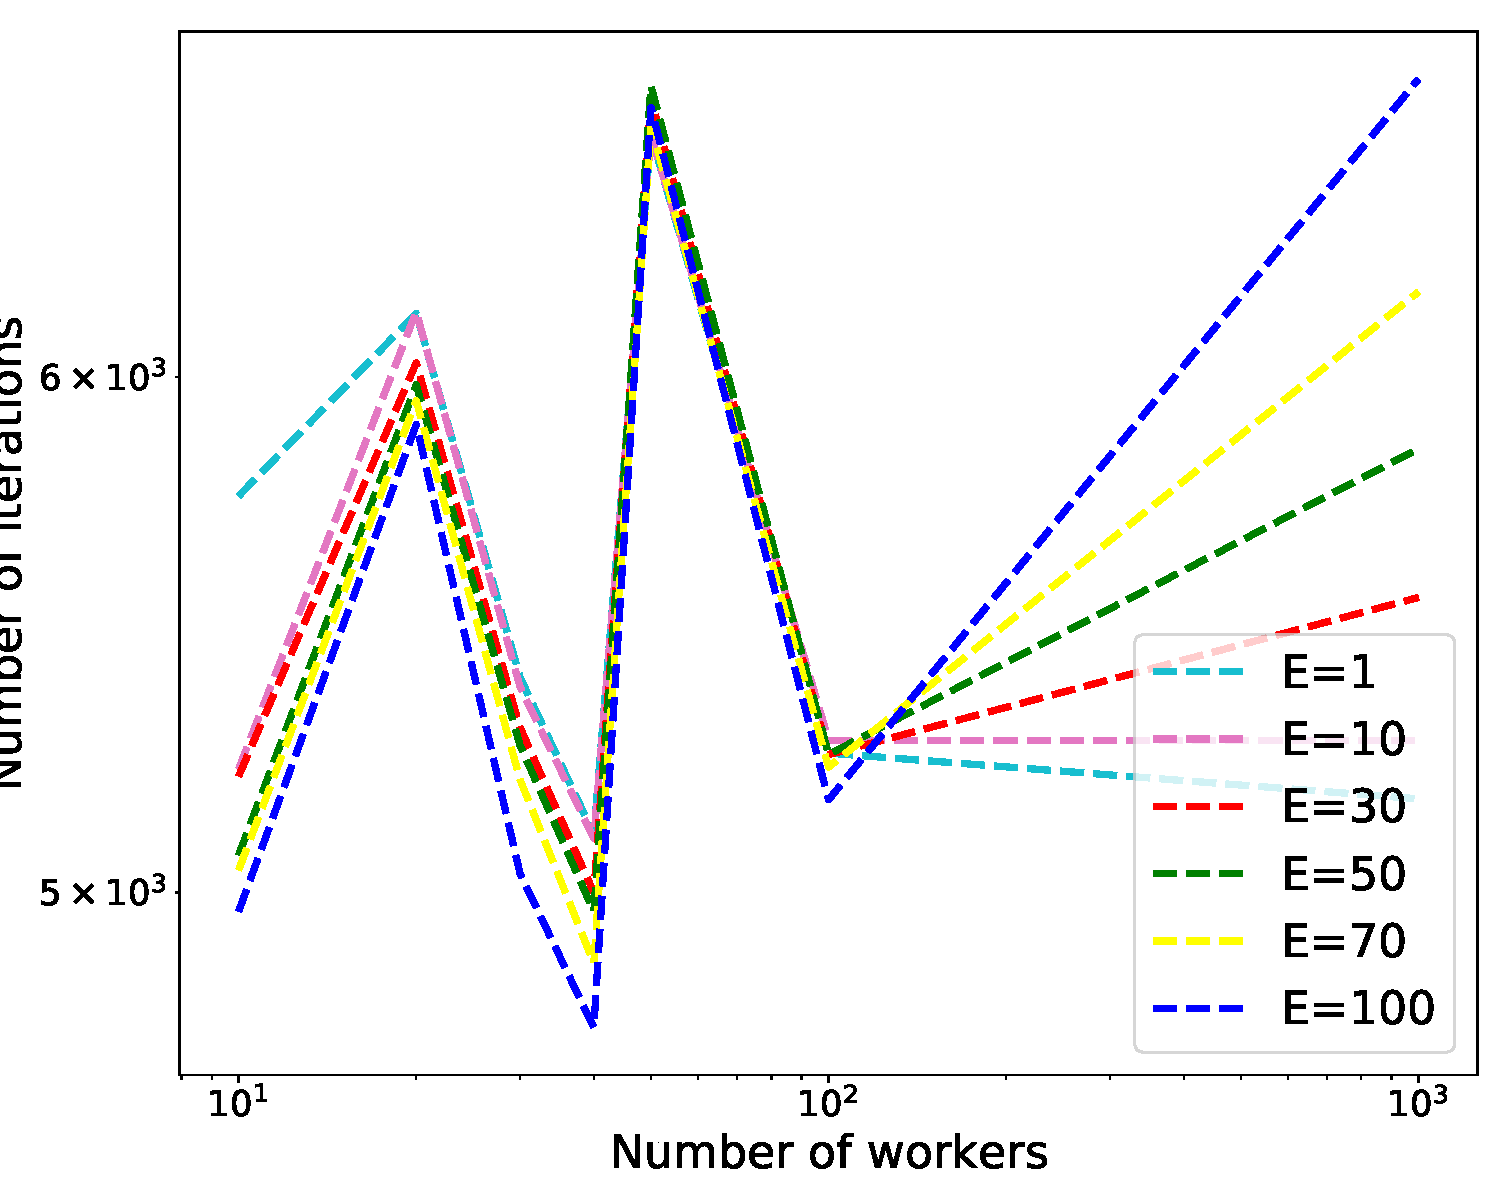
\includegraphics[width=0.5\textwidth]{fig/speedupNodesT-synthetic_logistic_regression_iclr300-epsilon07-b4-adapt0.pdf} & 
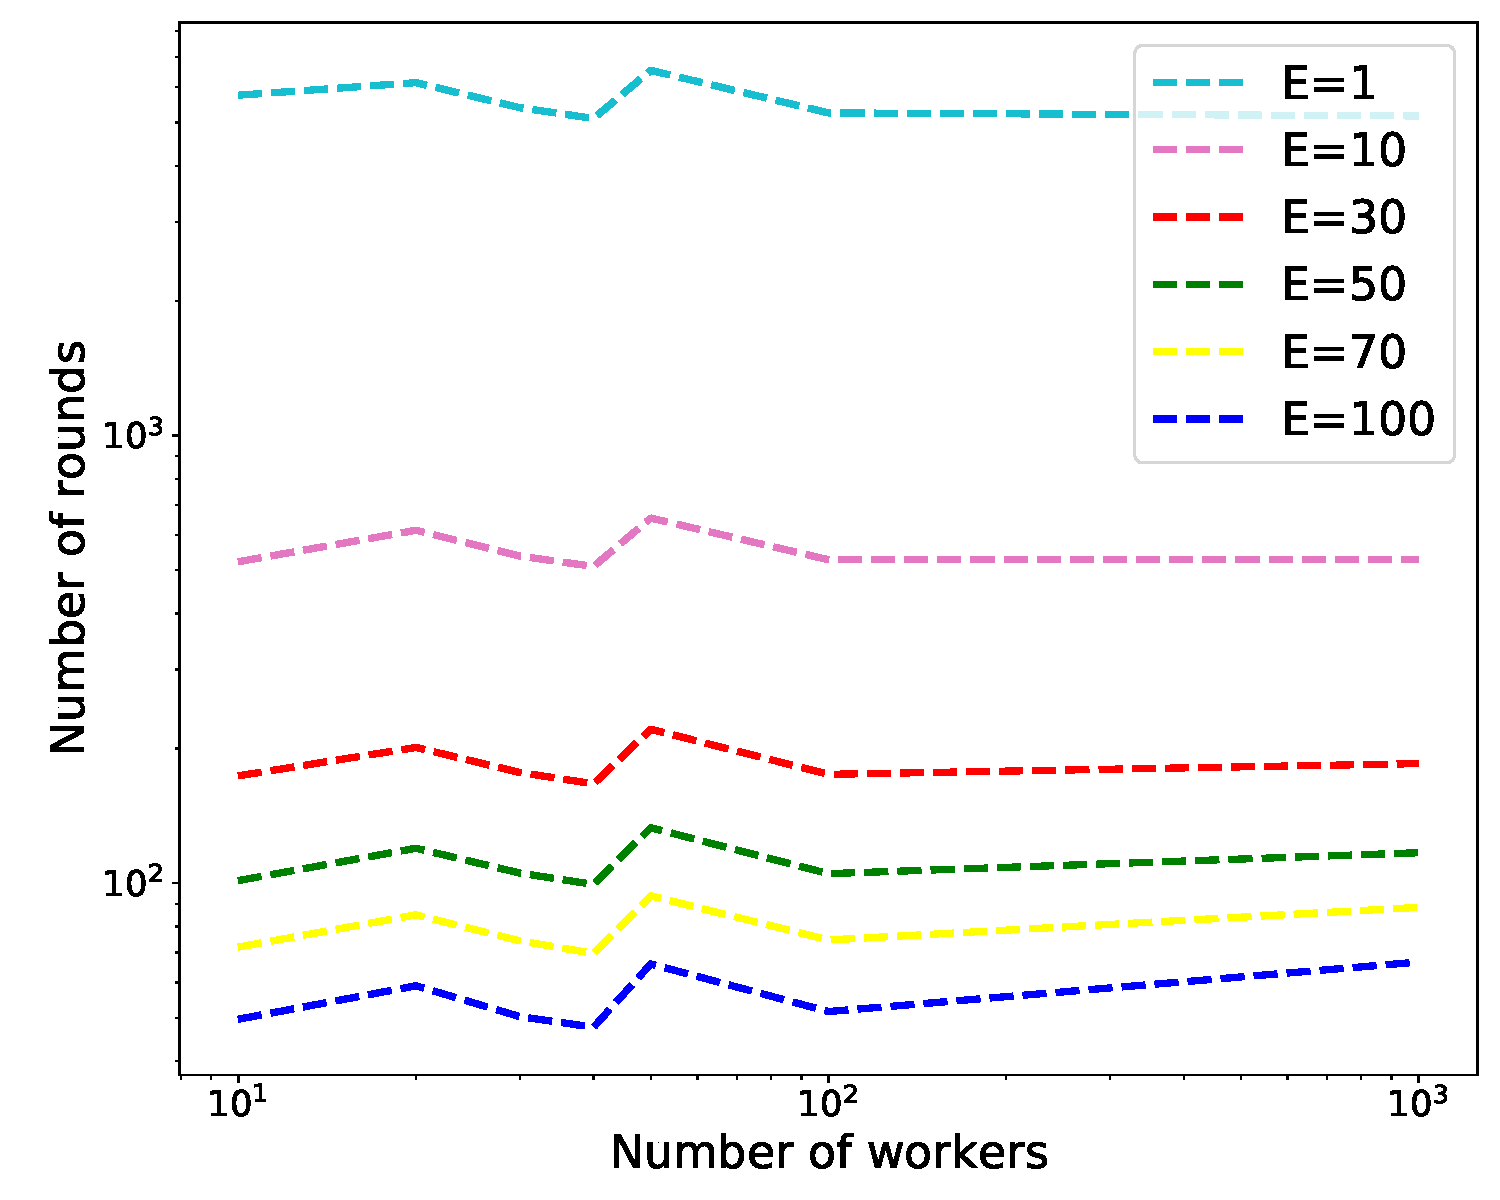
\includegraphics[width=0.5\textwidth]{fig/speedupNodesRounds-synthetic_logistic_regression_iclr300-epsilon07-b4-adapt0.pdf} \\
\end{tabular}
	\caption{Logistic regression with regularization $0.001$. The linear speed up w.r.t the number of nodes and number of epochs. The synthetic dataset has $42000$ samples, evenly distributed on $10, 20, 30, 40, 50, 100, 1000$ devices. The figure shows the number of iterations/rounds needed to converge to $\epsilon-$accuracy. The learning rate is decayed as the $\eta_t = \frac{1}{1 + t \times a}$, where we extensively search the best learning rate $c \in \{1, 10\}$ and $a \in \{1, 0.1, 0.01\}$ for each configuration. Batch size is 4 in this case.}
\end{figure}



\begin{figure}
\centering
\begin{tabular}{cc}
	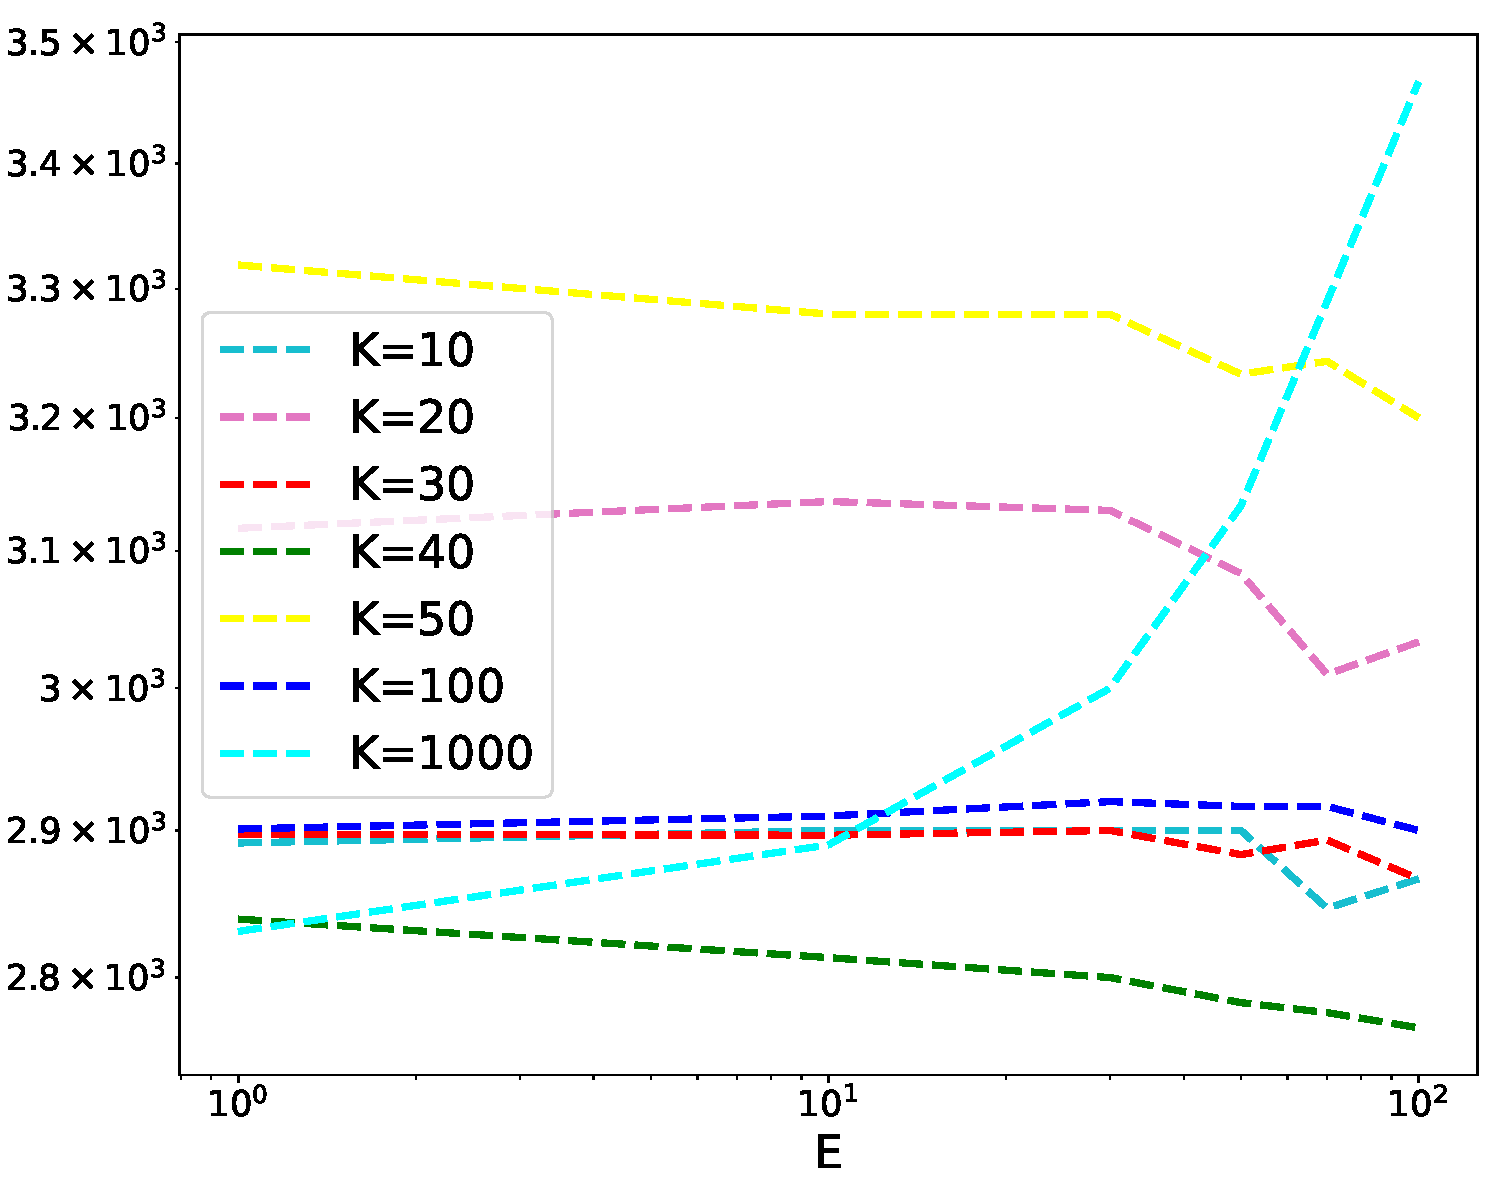
\includegraphics[width=0.5\textwidth]{fig/speedupEpochsT-synthetic_logistic_regression_iclr300-epsilon07-b4-reg0-adapt0.pdf} & 
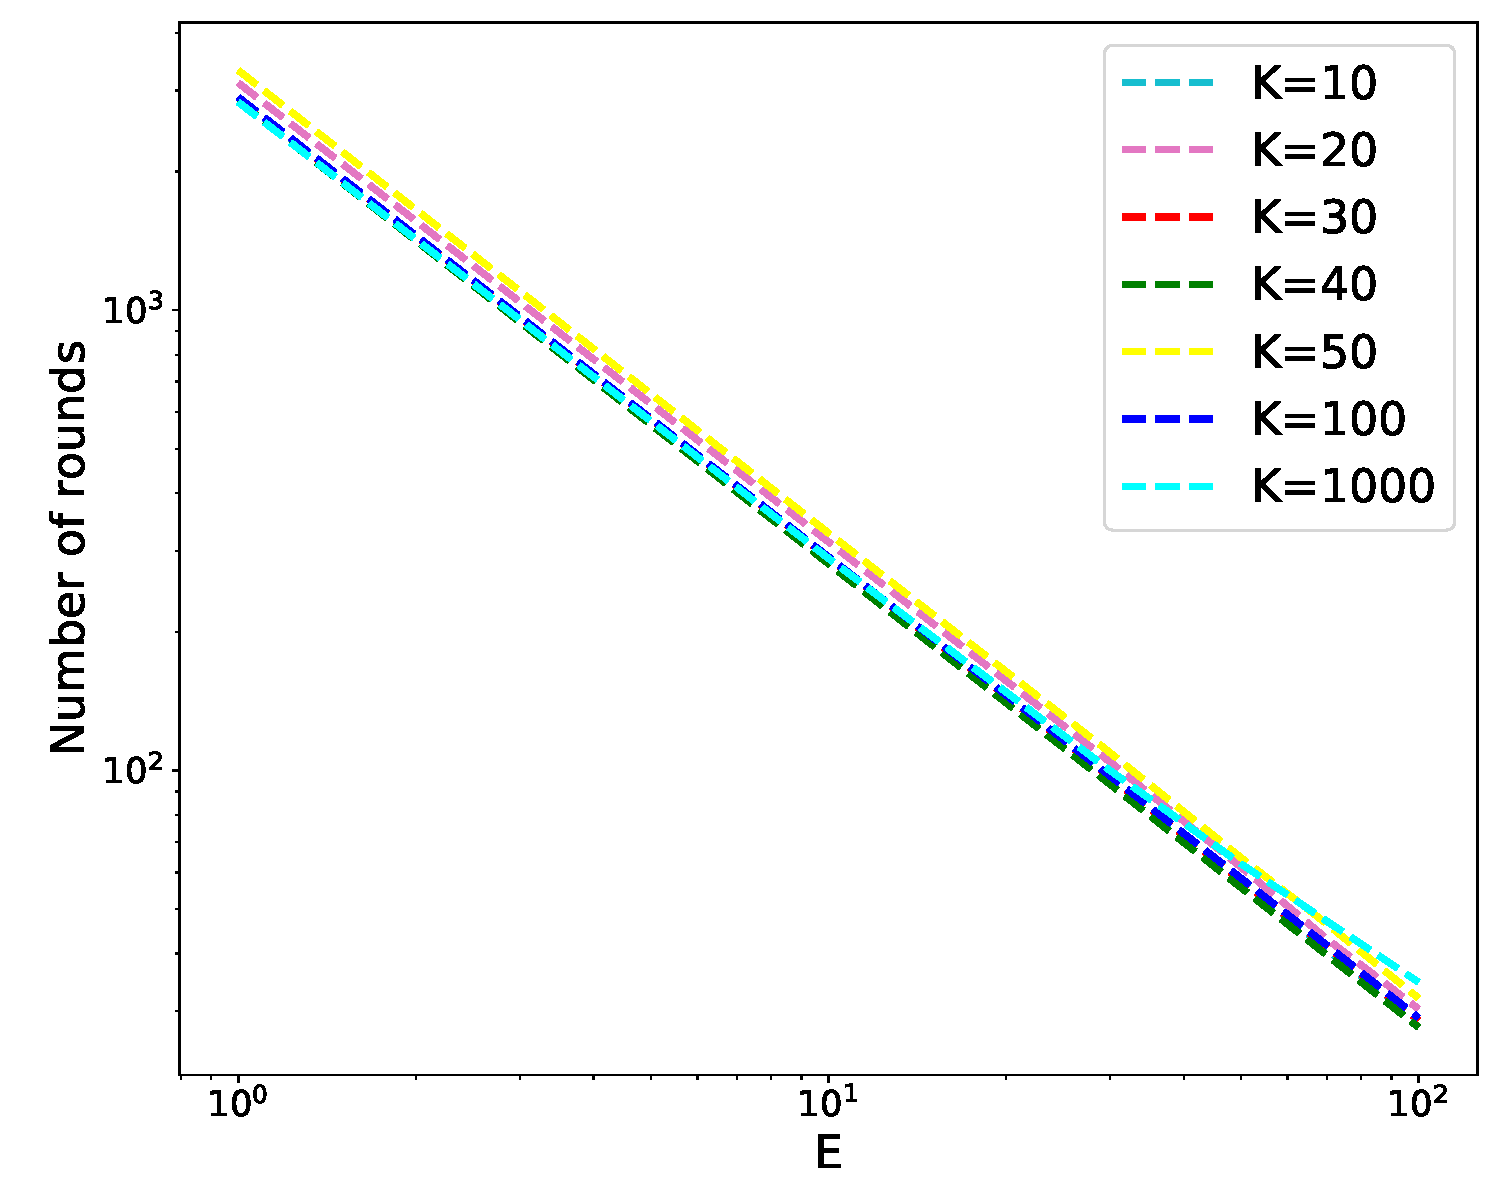
\includegraphics[width=0.5\textwidth]{fig/speedupEpochsRounds-synthetic_logistic_regression_iclr300-epsilon07-b4-reg0-adapt0.pdf} \\
	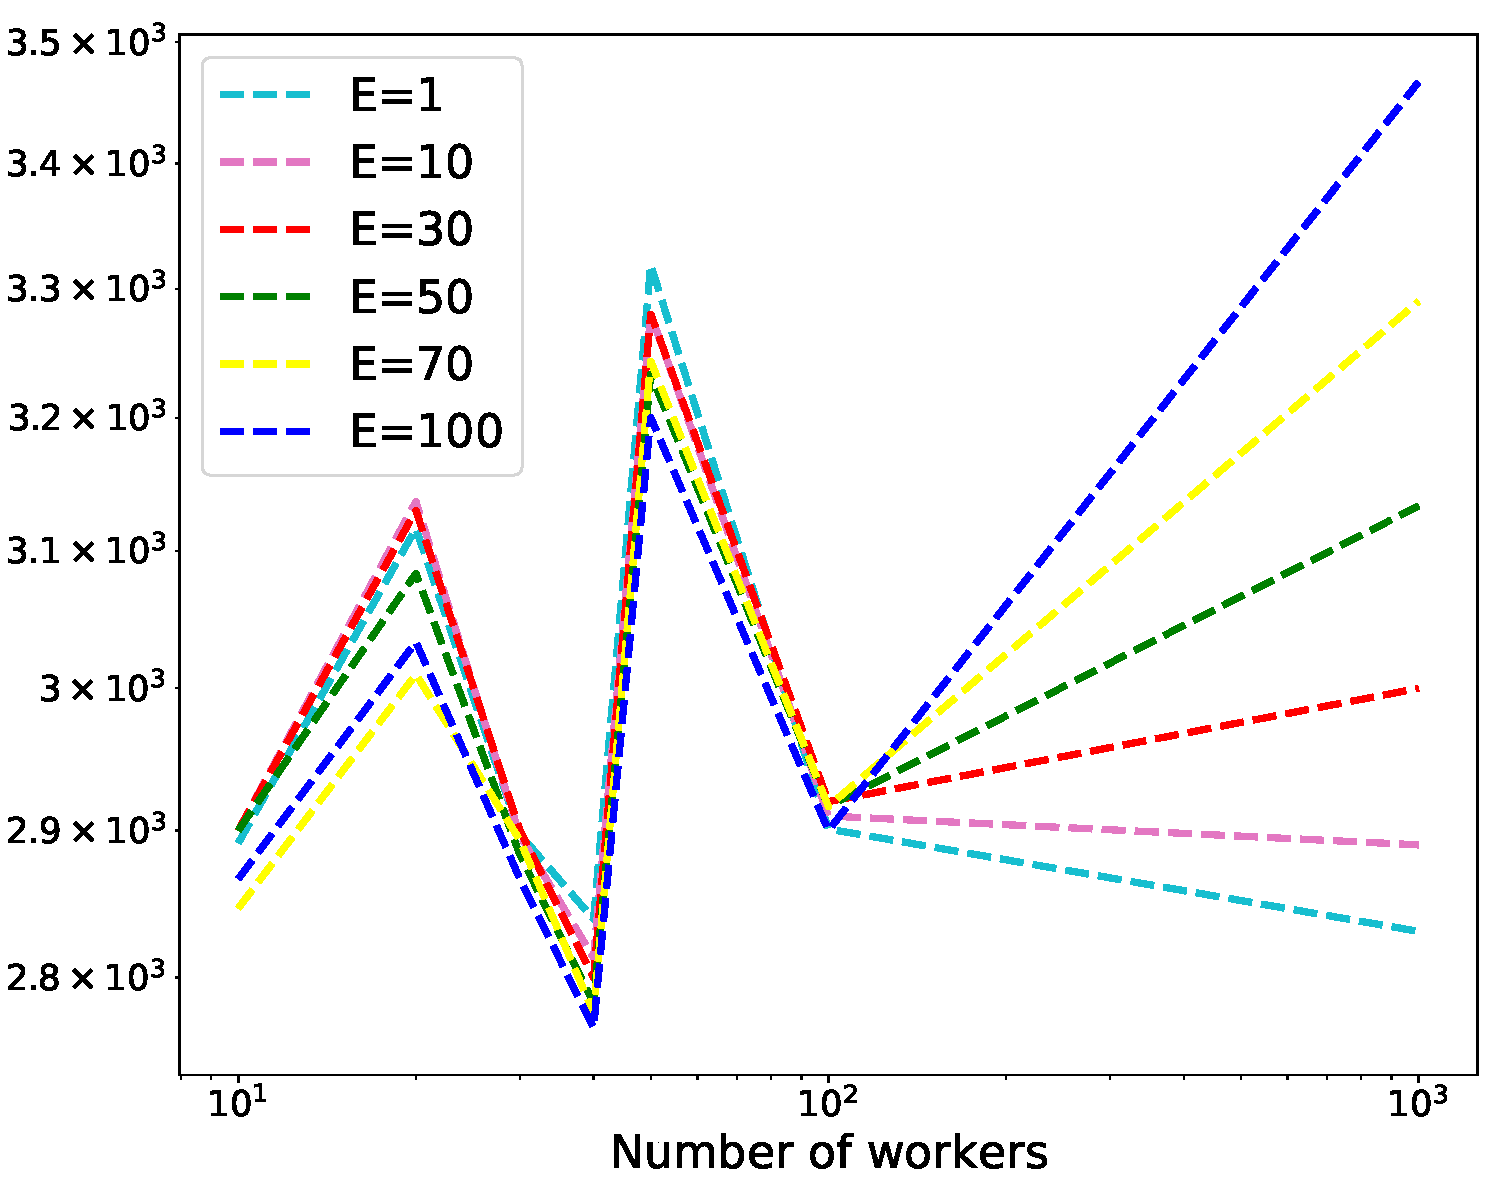
\includegraphics[width=0.5\textwidth]{fig/speedupNodesT-synthetic_logistic_regression_iclr300-epsilon07-b4-reg0-adapt0.pdf} & 
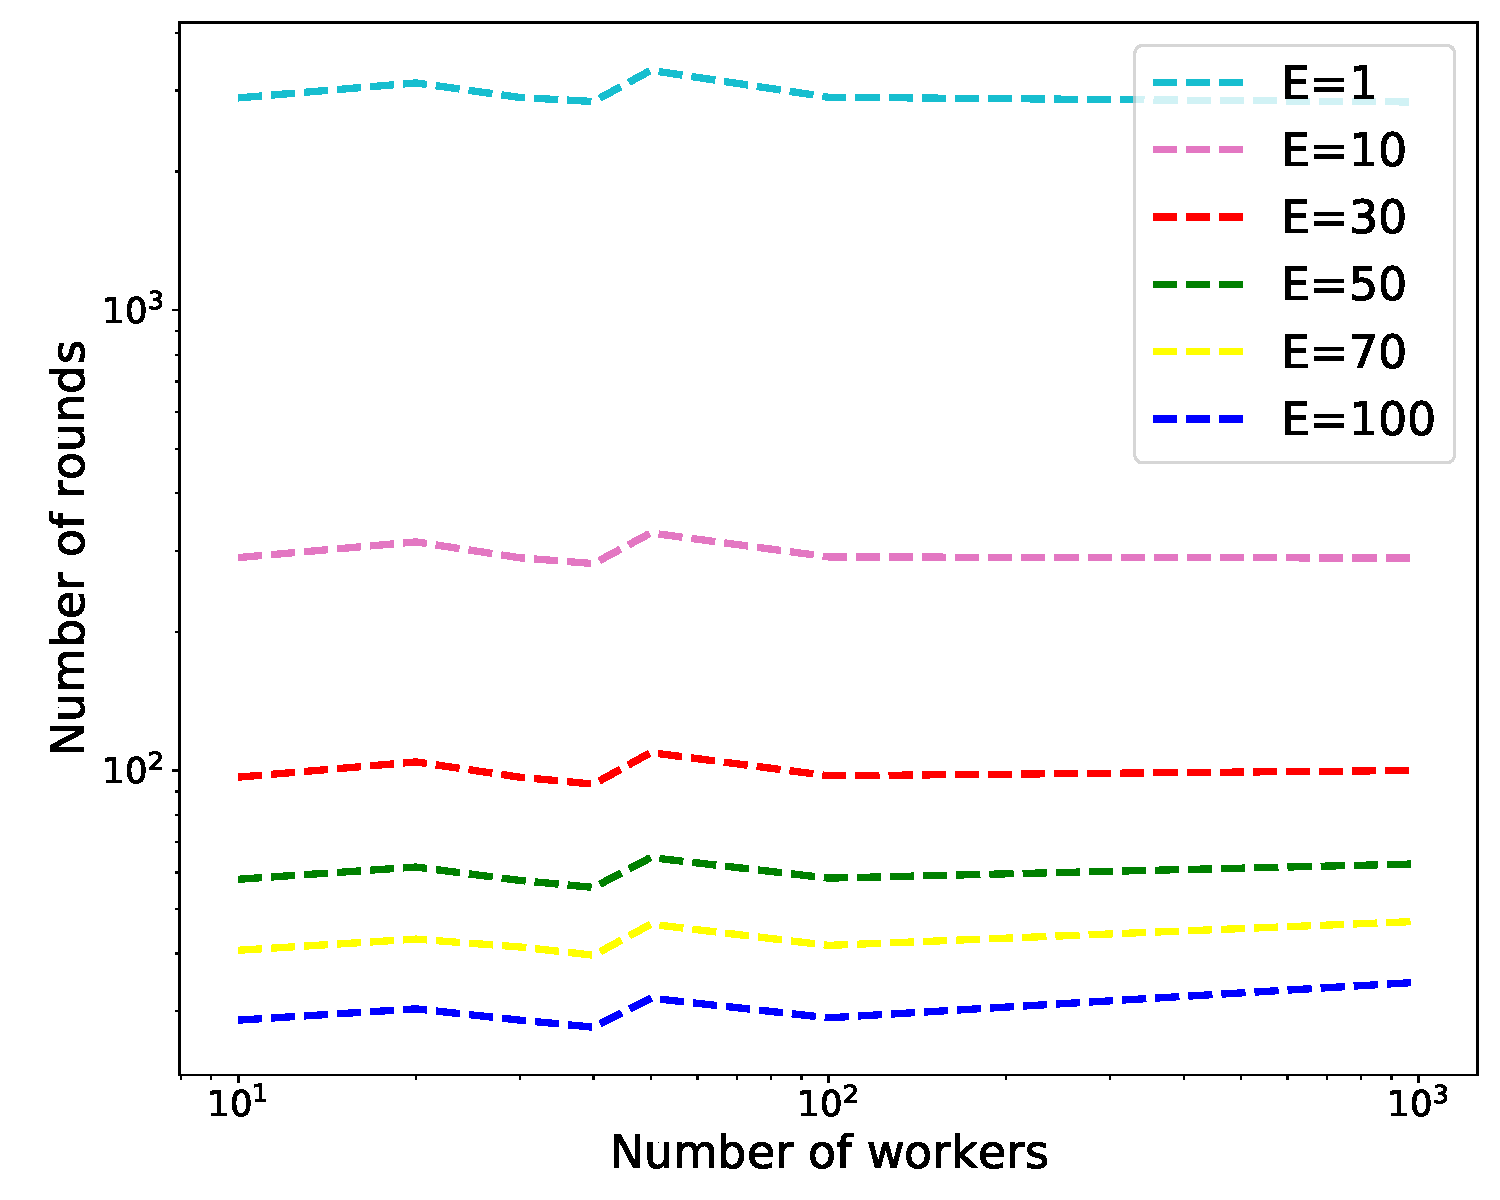
\includegraphics[width=0.5\textwidth]{fig/speedupNodesRounds-synthetic_logistic_regression_iclr300-epsilon07-b4-reg0-adapt0.pdf} \\
\end{tabular}
	\caption{Logistic regression with regularization $0$. The linear speed up w.r.t the number of nodes and number of epochs. The synthetic dataset has $42000$ samples, evenly distributed on $10, 20, 30, 40, 50, 100, 1000$ devices. The figure shows the number of iterations/rounds needed to converge to $\epsilon-$accuracy. The learning rate is decayed as the $\eta_t = \frac{1}{1 + t \times a}$, where we extensively search the best learning rate $c \in \{1, 10\}$ and $a \in \{1, 0.1, 0.01\}$ for each configuration. Batch size is 4 in this case.}
\end{figure}


% /media/Research/linkaixi/env/py36/bin/python /home/linkaixi/Dropbox/recsys/convexFed/main.py --dataset=synthetic_logistic_regression_small --epsilon=0.01 --num_rounds=500000 --num_epochs=1 --number_user=10 --learning_rate=0.001 --is_decay=True --lrconst=1 --machine=gpu --batch_size=4 --num_iteration=50000 --model=logisticregression --optimizer=fedave --dimension=60 --adapt=0
% \subsection{Nesterov}
